% Chapter Template

\chapter{Introduction} % Main chapter title

\label{ch:intro} % Change X to a consecutive number; for referencing this chapter elsewhere, use \ref{ChapterX}


%% =====================================================================================
%%
%%               I N T R O D U C T I O N
%%
%% =====================================================================================

%% From Just
A pair of massive stars at the end of their evolution, undergo \ac{SN} explosion, forming, 
in certain cases, a pair of compact objects orbiting each other. A particular interesting 
example is a pair of \acp{NS}, compact, but heavy objects sustained against gravitational 
collapse by the neutron degeneracy pressure. The theory of \ac{GR} predicts that the orbit 
of the system shrinks, as \acp{NS} loose energy and angular momentum to \acp{GW}. The 
loss continues until \acp{NS} collide at their last orbit a form an axisymmetric object.
In this thesis we investigate such a merger, focusing on the aftermath evolution of the 
remnant. 

The high compactness of \acp{NS} lead to an energetic, explosive merger, where a certain
fraction of the \ac{NS} matter is ejected from the system at mildly relativistic 
velocities. In addition to the complex dynamics of the system after merger that might 
induce additional matter outflows, this makes the \ac{BNS} mergers a strong contributor 
to the cosmic chemical evolution. The matter ejected at/after mergers, \ie, ejecta, has 
unique properties, rarely found in other astrophysical cites. Specifically, the abundance 
of free neutrons allow for the so-called rapid neutron capture process,
the \rproc{}, that is responsible for the production of the heaviest elements in the 
Universe, lanthanides and actinides. 

Wide range of possible types and properties of ejecta lead to a similarly broad 
range in \ac{EM} counterparts to \ac{BNS} mergers. Perhaps, two of the most 
well studied ones are the \ac{kN}, a thermal counterpart powered by the decay of 
newly synthesized heavy elements in the ejecta, and \acp{SGRB}, generally non-thermal 
emission from the ultrarelativistic collimated outflow, formed after the merger. 
Study of these \ac{EM} counterparts in conjuncture with \acp{GW} emission allows to 
gain unique insigts into the inner workings of the \ac{BNS} merger and previously 
unobtainable constraints on the theory of gravity, the properties of matter at 
supranuclear densities, origin of the \ac{SGRB}, cosmic chemical evolution. 

The complexity, non-linearly, non-stationarity and multidimensionality of physical 
processes operating at \ac{BNS} mergers on a broad range of scales of length and time 
implies that self-consistent, quantitative studies are only possible with numerical 
simulations. These simulations, performed with numerical codes that took years of 
develop and test, are very computationally expensive, rare and require detailed 
postprocessing and analysis. Moreover, the self-consistent modeling of the merger and 
\ac{EM} counterparts is still beyond the reach of modern methods. Generally, the 
the short-term (hundred of milliseconds) evolution of the merger itself 
is handled with \ac{NR} codes while the \nuc{} and \ac{EM} emission are evaluated 
after, in postprocessing. Strengthening the connection between these methods is one of 
the goals of this thesis. 

In the following sections we sketch the astrophysical background to clarify the 
context of our study and we conclude the chapter by summarizing the main points of 
motivation for this thesis and its structural arrangement.


%% <<< From Radice Review >>>
\ac{BNS} mergers lie in the center of a variety of physical processes in astrophysics.
The first ever detection of such event by LIGO/Virgo \acp{GW} observatories and 
numerous \ac{EM} observatories, the \GW{} had significantly advanced our understanding 
of gravity, physics of dense matter, \acp{SGRB} and origins of \rproc{} elements 
\cite{1,2,3}. 
%
Detection and analysis of \acp{GW} from inspiraling \acp{NS} allows to asses 
the \ac{NS} \ac{EOS}, quantified by so-called tidal deformability, and as such, the 
properties of matter at supernuclear densities \cite{5,6,7}. Information about matter 
at densities several times that of the nuclear matter 
% and tepmteratures of tens of MeVs 
can be obtained from \acp{GW} emitted by the \acp{BNS} merger product \cite{8,9,10,11}. 
%
The conditions within the matter, ejected at mergers are sufficient for the \rproc{} 
\nuc{}, responsible for the production of the heaviest elements in the Universe
% such as gold 
\cite{12}. This was confirmed by \ac{MM} observations of \GW{} \cite{12}. 
% however, it is unclear whether \ac{BNS} mergers is the dominant source of 
% \rproc{} elements in the universe, or if other \rproc{} cites are required to 
% explain the observed abundances in the oldest stars, \ac{UFG} and our solar system. 

Single \acp{NS} are very compact object, where compactness 
$C_{i} = GM_i/R_i^2c^2\propto0.15$ and effects of \ac{GR} cannot be neglected 
when describing them. A pair of \acp{NS} orbiting each other slowly loses the 
angular momentum to \acp{GW}. The timescale for the radiation reaction, however, 
is much longer than the orbital period for most of the inspiral and the 
system evolution can still be considered adiabatic. 
% For instance, the inspiral can be considered as a sequence of circular orbits. 
% However, during last orbits before merger, the finite size (tides) and \ac{HD}
% effects starts to become important. 
The inspiral ends at the onset of the Roche lobe overflow, when the binary 
reaches the mass-shedding limit \cite{13}.

In order to study the dynamical phase of \ac{BNS} mergers and \pmerg{} evolution, 
sophisticated \ac{NR} simulations are required. Modern, state-of-the-art methods 
include full \ac{GR}; composition-dependent nuclear \ac{EOS} with finite-temperature 
effects, \ac{GRMHD}, advanced neutrino trasport (with varying degree of sophystication,
\cite{14, 15, 16, 17, 18, 19, 20, 21}.

In this thesis we perform \ac{NR} simulations of \ac{BNS} mergers, report on their 
qualitative and quantitative picture and its implication for the \ac{EM} signatures.
We focus on the nuclear astrophsyics aspect of the mergers, and on the comparison 
between theoretical predictions and observations of \GW{}, discussing the 
\rproc{} \nuc{}, thermal \ac{EM} transient, and non-thermal \ac{EM} afterglow. 

For the general overview on the topic we refer to \cite{22},
For the most recent reviews on the topic we recommend the following reviews:
Radice, for the discussing of the \pmerg{} dynamics and ejecta,
Bernuzzis, for the \ac{GW} aspect of the mergers \cite{Bernuzzi}
Shibata & Hotokezaka for the discussing of the ejecta \cite{Shibata & Hotokezaka}.
For more detailed discussion on \ac{EM} counterparts to mergers we refer to \cite{23,24,25}.

This chapter is organized as follows...
First we discuss the observational context of the \ac{BNS} mergers, focusing on the 
ejecta \nuc{} and \ac{EM} counterparts.
Then we overview the current picture of \ac{BNS} mergers with emphasis on the 
\pmerg{} dynamics and mass ejection mechanisms. 
Finally, we state the goals of this thesis.




\section{Observational context}


%% =====================================================================================
%%
%%               N U C L E O S Y N T H E S I S
%%
%% =====================================================================================

\subsection{\rproc{} \nuc{}}\label{sec:nuc:rproc}

%It is of paramount importance for testing nucleosynthesis theories and models to have an 
%accurate measurements of relative abundances in the Universe. For Humanity, confined 
%still to just one planet, this is not a trivial task. And while automatic spacecrafts, 
%such as Luna, Apollo and Hayabusa have delivered samples from asteroids, most of the 
%studies are performed using the naturally falling meteorites. The composition of these 
%guests from space is then thoroughly studied via absorption and emission spectroscopy 
%\citep{Shaviv:2012}.
%
%The understanding of the solar system isotope and element abundances have come a long way 
%\citep[\eg][]{Cameron:1973,Anders:1989,Grevesse:1998,Lodders:2003} 
%%%%\textcolor{red}{add last papper you used for solar A.}

\begin{figure}[t]
    \centering
    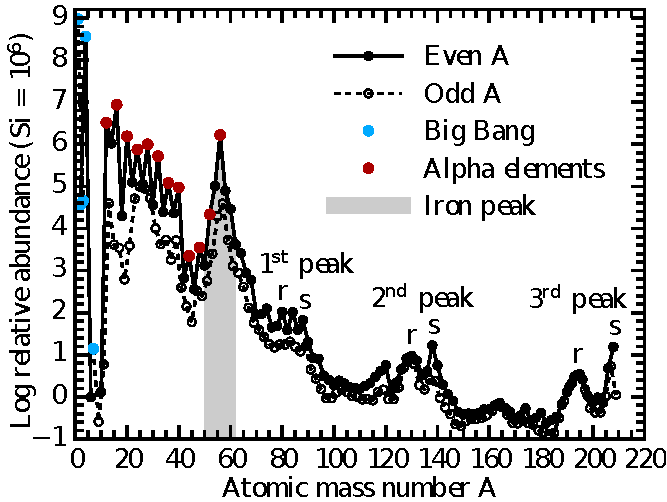
\includegraphics[width=0.49\textwidth]{Fig_1_1_Lip.pdf}
    \caption{Observed abundances in our solar system as a function of mass number
        $A$. The lightest elements were created in the Big Bang and fusion in stars predominantly
        creates alpha elements. The iron peak is made in core-collapse and type
        Ia \acp{SN}. Elements beyond the iron peak are synthesized by the slow ($s$) and
        rapid ($r$) neutron capture processes. These processes produce three distinct double
        peaks. Abundance data from \citet{Lodders:2003}. (Adapted from \citet{Lippuner:2018phd})
    }
    \label{fig:nuc:fig11_lip}
\end{figure}

%\begin{sidenote}
%    \textcolor{red}{Figure with solar observed abundances, showing $r$-elements and $s$-elements}
%    The observed obundacnes as a function of atomic mass number $A$ are shown in figure Fig. (XXX). 
%(data from \cite{Lodders:2003}). The plot shows nuclei that are more bound (due to spin pairing of nucleons 
%\cite{Moller:1993ed}), \textit{i.e,} those with an even $A$ number, are more abundant. The lowest binding 
%energy of nuclei with odd number of neutrons and protons (but even $A$) are largely unstable or short-lived. 
%A few exceptions are \textit{e.g.,} $^{40}$K, $^{50}$V, $^{138}$La and $^{176}$Lu, 
%that have a half-life of at least $10^{9}$ years.
%\end{sidenote}

The dominant \nuc{} process, responsible for the production of elements, varies with the mass 
number $A$.
%
For instance, light elements $A<8$ were synthesized right after the Big Bang
in the process known as \ac{BBN}.
Nuclides before the iron peak, $12\leq A\leq 56$ come from stellar hydrostatic 
nuclear burning \citep[\eg][]{Rolfs:1988,Hasen:2004}.
Elements at the iron peak $50\leq A \leq 62$ produces mostly 
during the type Ia \acp{SN} or explosive silicon burning in \acp{CCSN} \citep[\eg]{Woosley:2002}. 
The conditions at these sights are such that the dense material at the \ac{NSE}\footnote{
    At \ac{NSE} three parameters describe the composition: 
    density, temperature and electron fraction $Y_e = n_p/(n_p + n_e)$, 
    where $n_e$ and $n_p$ are the (total) number density of electrons and protons 
    respectively \citep{Seitenzahl:2009}. 
    The composition at \ac{NSE} favors more tightly bound nuclides,
    as they are more difficult to photodissociate.
}, 
expands and cools down, enriching the \ac{ISM} with heavy elements \citep{Iwamoto:2000as}. 
%
%Most of the material beyond iron peak are produced via neutron capture processes 
%\citep{Burbidge:1957}.
Nuclides with $A\geq 56$ cannot be synthesized via standard cycles due to their 
strong Coulomb barriers. 
Thus, processes that do not involve charged particles become dominant. 
These are the neutron capture processes \citep{Burbidge:1957}.


%% -------------------------------------------------------
%%                   Nucleosynthesis Cites
%% -------------------------------------------------------

%\subsection{Nucleosynthesis up to the iron peak}
%
%
%\subsubsection{Big Bang nucleosynthesis}
%
%Light elements in the Universe, like hydrogen ($\sim 75\%$ by mass) and helium 
%($\sim 25\%$ by mass) alongside trace amounts of $^{3}$He and $^{7}$Li were created 
%during the \ac{BBN} (see \eg, \citet{Tytler:2000qf} and references therein). 
%And while only a small number of nuclides were involved in \ac{BBN}, 
%there are large discrepancies between \ac{BBN} models and observations. 
%For instance, the "lithium problem" \citep{Coc:2013eha}, which origin is not well 
%understood \citep{Fields:2011zzb}.
%
%
%\subsubsection{Low-mass stellar burning}
%
%In order to fuse massive nuclides and overcome the strong Coulomb barrier, high temperatures, 
%($\geq 10^6$ K) are required. Thus production of heavy elements from hydrogen and helium 
%is possible only in special environments, in particular, in the interior of stars 
%\citep{Bethe:1939}. 
%For the most of their lives stars burn hydrogen into helium. The process releases the 
%binding energy and maintains the hydrostatic stability of a star. After the hydrogen is 
%exhausted in the core, a core (atmosphere) contracts (expands), heats up (cools), and the 
%shell hydrogen burning is initiated, slowly depositing ashes, \eg, helium, into the inert core. 
%The star's subsequent evolution depends primarily on its mass. If the mass of a star 
%$M>0.5M_{\odot}$, at some point the helium in the core starts to fuse into $^{12}$C and 
%$^{16}$O and small amounts of $^{24}$Mg, $^{28}$Si. These elements are called 
%\textit{alpha elements} \citep{Rolfs:1988,Hasen:2004}. 
%The end of the core helium burning phase leads to another core contraction phase. 
%A star of a mass $\sim 8M_{\odot}$ would be able to ignite carbon and oxygen producing 
%heavier elements afterwards. A less massive star looses its outer layers and becomes a 
%slowly cooling degenerate core, a white dwarf.
%
%
%\subsubsection{nuclear burning is massive stars}
%
%For a star that has $M\geq 8M_{\odot}$, a sequence of burning stages follows, each of 
%which leads to the exhaustion of a respective fuel, contraction of the core and rise of 
%its temperature \citep{Woosley:2002}. Carbon burning leads to the production of 
%$^{20}$Ne, $^{23}$Na and free protons that contribute to the synthesis of non-alpha elements. 
%As temperature increases, the photodisintegration of $^{20}$Ne becomes possible and a small 
%amount of $^{24}$Mg is formed. Next, the oxygen burning occurs producing $^{28}$Si $^{31}$P, 
%and $^{28}$Si and $^{32}$S, that become dominant nuclides in the core by the end of oxygen burning \citep{Rolfs:1988}.
%
%The subsequent silicon burning proceeds at $T\sim3.5\times10^9$K through photodissociation 
%of some of the $^{28}$Si and a sequence of alpha particle captures, "alpha ladder", on the 
%remaining $^{28}$Si to form $^{32}$S, $^{36}$Ar, $^{40}$Ca, $^{44}$Ti, $^{48}$Cr, $^{52}$Fe 
%and $^{56}$Ni. This process lasts around a day \citep{Rolfs:1988,Hasen:2004}. Due to high 
%temperatures present at silicon burning, nuclides with $A\in[28, 62]$ fall into quasi-equilibrium, 
%meaning that these nuclides (with exception of $^{12}$C, $^{16}$O $^{20}$Ne and $^{24}$Mg), 
%alpha particles and protons participating in reactions, are in equilibrium with each other. 
%
%At $A=56$ the binding energy per nucleon appears reaches its maximum and the silicon burning 
%cannot produce heavier nuclides with the release of energy. As the fraction of $^{56}$Ni in the 
%core of a star increases, the support that nuclear burning has provided against gravitational 
%contraction falls. Meanwhile the mass of the degenerate core still increases as burning proceed in shells.
%However, when the electron degeneracy pressure can no longer counteract gravity, \ie, when mass 
%of the core exceeds the effective Chandrasekhar mass\footnote{
%    The collapse however occur before the core reaches Chandrasekhar mass, and the pressure 
%    support that rests on the availability of free electrons drops when electrons capture on 
%    the nuclides becomes possible. To account for this, the effective Chandrasekhar mass was 
%    introduced.
%}, 
%the core collapses leading to a \ac{CCSN} \citep{Woosley:2002}.
%Thus, the origin of more abundant alpha elements in the Universe is stellar fusion.
%
%
%\subsubsection{Iron Peak}
%
%At temperatures higher then $T\sim 5\times10^{9}$K nuclear \ac{NSE} establishes. This is a 
%balance between the fusion reactions forming a ($N,Z$) nuclide from $N$ neutrons and $Z$ 
%protons and photodissociation reactions, splitting it back. 
%At \ac{NSE} three parameters describe the composition: density, temperature and 
%electron fraction $Y_e = n_p/(n_p + n_e)$, where $n_e$ and $n_p$ are the (total) 
%number density of electrons and protons respectively \citep{Seitenzahl:2009}. 
%%
%The composition at \ac{NSE} favors more tightly bound nuclides, as they are more difficult 
%to photodissociate. Thus, if the conditions allow, \ie, temperature, density and electron 
%fraction of the mater, ($Y_e \sim 0.46$, an electron fraction of iron), nuclides at $A\sim56$, 
%\ie, iron peak elements, dominate \citep{Seitenzahl:2009}. 
%%
%For example, \ac{NSE} establishes during the type Ia \acp{SN}, when a thermonuclear 
%explosion of a white dwarf allows for sufficiently high temperatures and densities. 
%After the explosion, newly synthesized elements of the iron peak cools, and being stable, 
%remain in the expanding medium \citep{Iwamoto:2000as}.
%
%
%\subsection{Nucleosynthesis beyond the iron peak}
%
%Nuclides with $A\geq 56$ cannot be synthesized via standard cycles due to their strong Coulomb 
%barriers. Thus, processes that do not involve charged particles become dominant. 
%These are the neutron capture processes.
%%
As nuclides absorb neutrons and grow larger, their binding energy, $Q_n$, decreases. This process 
is stopped when $Q_n\sim1$~MeV and energetic photons start to knock out neutrons from a nucleus. 
This process is called photodisintegration and a location in the parameter space where it occurs, 
(that in turn dependents on temperature and density), is called the 
%% [IMPORTANT]
neutron drip line 
%% ---
\citep{Rolfs:1988}.

Nuclides produced via neutron capture are generally unstable to $\beta$-decay, with a timescale, 
$\tau_{\beta}$, that can be larger or smaller than a neutron capture timescale, $\tau_n$. 
In case when $\tau_{\beta}\ll\tau_n$, \ie, when a $\beta$-decay occurs faster then the next 
neutron capture, the process is called \textit{slow} or \sproc{}. 
Thus, by definition, the \sproc{} moves along the valley of stability\footnote{
    a region of stable nuclides in the nuclides chart -- a chart in terms of number of neutrons $n_n$ 
    and number of protons $n_p$.
}, departing no further than by a few nuclides away.
On the other hand, if $\tau_{\beta}\gg\tau_n$, \ie, when a neutron capture occurs much faster then 
a $\beta$-decay, the process is called \textit{rapid} or \rproc{}. This \nuc{} generates nuclides 
near (but not crossing) the neutron drip line (See Fig.~\ref{fig:nuc:fig16_lip}) \citep{Rolfs:1988}. 

\begin{figure}[t]
    \centering
    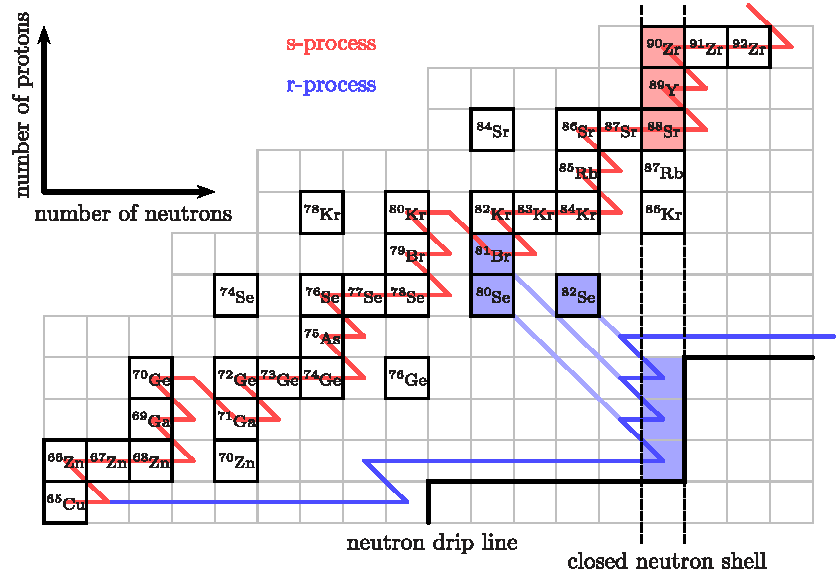
\includegraphics[width=0.60\textwidth]{Fig_1_6_Lip.pdf}
    \caption{Schematic representation of the $s$- and $r$-process on a section of the
        chart of nuclides. The s-process (red) proceeds along the valley of stability and the
        r-process (blue) along the neutron drip line. At the closed neutron shell N = 50, the
        neutron capture cross section drops by several orders of magnitude, which leads to a
        pile up of material there that produces the double-peak features
        (Adapted from \citet{Lippuner:2018phd})
    }
    \label{fig:nuc:fig16_lip}
\end{figure}
%
%% --- IMPORTANT --- ORIGIN OF THE PEAKS IN r-PROCESS
Notably, the trajectory of $r$-process is interrupted when the neutrons within a nuclide can arrange 
themselves in a closed shell. Such configurations are energetically very favorable and thus the cross 
section for a subsequent neutron capture reduces. Only after several $\beta$-decays does the 
$r$-process continue. Thus, nuclides located at points where neutron drip line and closed neutron 
shell overlap is more abundant. These unstable nuclides will decay back to the valley of stability 
and some of the neutrons within them turn to protons, reducing the total mass of them. The indication 
of this "overproduction" are the peaks in the abundance patterns at a mass, $A$, slightly lower then 
the one corresponding to a closed shell nuclide (see Fig.~\ref{fig:nuc:fig11_lip}).


%%% --- important
A similar "overproduction" of nuclides with a closed neutron shell occurs when an $s$-process 
is considered. However, in that case it is caused by the cross section of these nuclides being 
$1-2$ order of magnitude smaller then of neighboring ones \citep{Rolfs:1988}. Thus, in the case of 
\sproc{}, the peaks in abundance pattern will be at $A$, corresponding to the closed shell exactly, 
and thus located at larger $A$ than that of the \rproc{}. Closed shell nuclides are located at 
$N=50,\: 82, \: 126$ and thus corresponding abundance peaks for $s$-process are at 
$A=88, \: 138, \: 208$ and at $A=80,\:130,\:194$ for $r$-process (see \eg, \citet{Arnould:2007gh}) 
(See peak structure in Fig.~\ref{fig:nuc:fig11_lip}).

%% --- Motivation MP stars --- THE GENERIC SOLAR ABUNDANCES
It was found, that the solar \rproc{} abundance pattern is consistent, and can be found anywhere in the 
Universe. In particular, in stars that were formed very early on a galactic evolution timescale, the 
\ac{MP} halo stars, one would expect to observe less \sproc{} and \rproc{} elements as there might have 
been not enough time for the enrichment to take place. However recent studies showed that the solar 
\rproc{} abundances are present in these stars as well \citep{Sneden:2008,Roederer:2010}, 
see also Fig.~$8$ in \citet{Sneden:2009}. Thus, modeling the \rproc{} \nuc{} it is expected to 
reproduce the solar abundances.

%%% -- can be deleted
%It is important to note that in addition to \sproc{} and \rproc{}, a possible $i$-process, (intermediate) 
%is widely discussed. The process operates further from the valley of stability than \sproc{}, but not 
%reaching neutron drip line \citep{Cowan:1977,Bertolli:2013gka}. Slow and intermediate neutron capture 
%processes operate within the low-mass \ac{AGB} stars with mass $M\in[1.5,3]M_{\odot}$ and more massive stars,
%that enrich the interstellar medium with heavy elements via strong winds 
%\citep[\eg][]{Peters:1968,Couch:1974,Kaeppeler:1994K,Woosley:2002,Straniero:2005hc,Herwig:2011}. 
%The possible cites for the \rproc{} we discuss in the following subsections.


\subsubsection{Possible $r$-process sites}

Study of possible cites of \rproc{} is a wide and rapidly developing field. The general requirement 
for \rproc{} is a low electron fraction, or, in other words, neutron-rich conditions. These can be 
found in a various places for certain models of Big Bang, that include inhomogeneities, 
\ac{BNS} and \ac{NSBH} mergers and \ac{SN} ejecta (see \citet{Mathews:1990} and references therein). 
%
Spectral studies of \ac{MP} stars (formed early in the galactic history), combined with models of 
galactic chemical evolution sheds light on possible dominant cite of \rproc{} material. 
\textcolor{red}{add more sources/models}. 
It is now believed that certain types of \acp{SN} and \ac{BNS} mergers are the most likely 
sources on \rproc{} material \citep{Mathews:1990,Thielemann:2011} \textcolor{red}{add more sources}


%\subsubsection*{\acp{CCSN}}

Collapse of a massive star produces a hot neutron core, that undergoes deleptonization, releasing 
$\sim10^{53}$~erg of binding energy in form of strong neutrino flux. These neutrinos, irradiating 
dense medium around the core, can produce a \nwind{} \citep{Qian:1996xt}, that was suggested to be 
a promising cite for \rproc{} \citep{Woosley:2002,Wanajo:2006mq}. Later, it was shown however, that 
the electron fraction in the wind would be too high for a full \rproc{}, and only "light" heavy 
nuclide up to $A\sim130$ can be synthesized 
\citep{Qian:1996xt,Thompson:2001ys,Fischer:2010,Roberts:2010,MartinezPinedo:2012rb,Wanajo:2013} 
\textcolor{red}{add Perego:2017} 
%
It is important to note, in the proton-rich \nwind{} nuclides with $A\sim 100$ can be produces 
via so-called $\nu p$-process. The process relies on a creation of a free neutron from proton by 
an antineutrino capture. These free neutrons can then be captured by a seed nuclide, $^{64}$Ge seed 
nuclide and thus nuclides heavier then $^{64}$Ge can be created
\citep{Frohlich:2006,Pruet:2005qd,Wanajo:2010mc,Arcones:2012}
%
A full \rproc{} can be achieved in so-called magnetorotationally driven \acp{CCSN}. This is a rare 
type of \acp{CCSN}, where a core of the progenitor is rotating rapidly and is strongly magnetized. 
Induced by a magnetorotational processes \eg, magnetorotational instability, collapse is accompanied by a
formation of a collimated bipolar jet 
\citep{Wheeler:2000,Akiyama:2003,Burrows:2007yx,Mosta:2014jaa,Mosta:2015} \textcolor{red}{add Siegel2019?.}.
Materiel in these jets is predicted to be sufficiently neutron rich to allow for a full \rproc{} 
nucleosynthesis \citep{Winteler:2012,Nishimura:2015nca}. The rarity of this type of \acp{SN}, 
however, might not allow it to be the dominant source or $r$-process material \citep{Nishimura:2015nca} 
(\red{See however Seigal:PAPER}). 


%\subsubsection{Compact object mergers}
\red{TO BE REWRITTEN -- REPETITION OF PREVIOUS CHAPTERS}

%% --- MIGHT NEED TO BE SHORTENED A LOT!  OR MOVED TO INTRODUCTION!
Mergers of two \acp{NS} or a \ac{NS} and a \ac{BH} are regarded as one of the main cites 
of \rproc{} material \red{list of refs}. Compact objects, formed in a binary evolution of massive stars, 
orbit each other for gigayears, before slow loss of energy from the system due to \acp{GW} 
reduces their orbit and they merge \citep[\eg][]{Hulse:1975,Lattimer:2004sa,Price:2006fi}. 
%
%The late inspiral and merger of \ac{BNS} or a \ac{NSBH} have been studied extensively via smooth particle 
%simulations \red{[REFS]} \ac{HD} simulations \red{[REFS]} and \ac{NR} simulations with simplified gravity \red{[REFS]} 
%or full \ac{GR} \red{[REFS]}. The composition of a \acp{NS} in these simulations have been modeled with 
%simplified polytropic \red{[REFS]} or piece-wise polytropic \red{[REFS]} or microphsyical \acp{EOS} \red{[REFS]}. 
%The physical setup of these simulations have also evolved to eventually include effects of
%neutrino radiation transport \red{[REFS]} and magnetic fields \red{[REFS]}. 

%These studies have shown that shortly before and during the merger, the neutron star(s) undergo(s) a tidal 
%deformation and disruption. Streams of neutron-reach matter are then ejected into the circombinary 
%with enough energy to be not graviationally bound to the system \citep{Price:2006fi,Foucart:2014nda,Sekiguchi:2015dma,Kyutoku:2015gda,Radice:2016dwd}. 

%% For details on the ejecta from \ac{BNS} mergers see Chapter \ref{ch:BNS_results}.
%% In addition, in case of a \ac{BNS}, when \acp{NS} collide, material at the collision interface, heated by shocks, 
%% gets 'squeezed' and launched in the directions perpendicular to the plane of the binary \cite{Bauswein:2013,Hotokezaka:2013b} \red{[REFS]}. 
%% Generally, these tow components, tidal and shocked, constitute the \textit{dynamical ejecta}. Where the term 
%% ejecta referrers to the material that has enough energy to leave the system. 
%% The properties of the dynamical ejecta from BNS have a broad distribution, especailly in terms of mass and ejectron fraction 
%% [\red{[REFS]} \& myFitPaper], where the former lies in range $(10^{-4},10^{-2})M_{\odot}$ and the latter $(0.05,0.45)$. 
%% We discuss dynamical ejecta properties of BNS in more details in section \red{sec:results:dyn\_ej:prop} and nucleosynthesis 
%% in it in \red{sec:results:dyn\_ej:nucleo}. In case of NSBH the ejecta mass was shown be larger, reaching $0.1M_{\odot}$ with 
%% low electron fraction, $\leq0.2$ but it requires that masses of BH and NS are comparable and BH is rapidly spinning 
%% \cite{Foucart:2014nda}\red{[REFS]}. If the BH is much more massive then NS, the latter would be 'swallowed' with no ejecta \red{[REFS]}.
%% After the merger, there are expected to be additional ejecta. For general postmerger configuration consists of a remnant, massive neutron 
%% star (MNS) or a black hole sorrounded by a disk (torus) of bounded matter. In the first case,  a strong neutrino flux from cooling MNS and 
%% disk can drive an outflow in the direction, perpendicular to the plane of the binary, the so-called \nwind{} 
%% (see Figure 1 from \cite{Perego:2014fma}) \red{[REFS],Jujibayashi+20}. This ejecta is expected to occure on a timescales of 
%% $\sim100$ms postmerger, be not very neutron rich $Y_e\sim(0.2-0.45)$ due to neutrino irradiation and have a mass of 
%% $(10^{-4}-10^{-3})M_{\odot}$ \red{[REFS]}. 
%% The massive nutron star born in a merger exhibit dynamical oscillations \red{[REFS]}. The $m=1$ mode, so-called 
%% "one-armed spiral instability" especially can persisit on a $\sim100$ms powtmerger timescale and become a dominant mode 
%% \red{[REFS], MainPaper}. This oscillations can inject energy within the disk, where via angular momentum transport it leads 
%% to an outer part of the disk to become unbound. This ejecta, the \textit{\swind{}} was shown to occur in all cases where the MNS is present. 
%% It has high electron fraction and its mass depends on a lifetime of the remnant, and for a $\sim100$ms it can amount to a few 
%% $\times\sim10^{-2}M_{\odot}$ \red{[Letter, MainPaper]}. We discuss the mechanism that drives the \swind{} in the section 
%% \red{sec:results:swind:mechanism} and the ejecta properties in \red{sec:results:swind:prop} and corresponding 
%% nucleosynthesis in \red{sec:results:swind:nucleo}.
%% On a longer timescales, the viscous processes and alpha recombination in the disk, surrounding MNS or a BH are expected 
%% to unbind additional material. This is so-called \textit{secular ejecta}. It is expected to be massive and neutron rich. 
%% However, due to long timescales involved, it is very difficult model \red{[REFS]}.

\ac{BNS} and \ac{NSBH} mergers eject neutron rich material (see chapter~\ref{ch:bns_sims}) 
in which \rproc{} can take place, producing nuclides beyond $A=300$. Over-saturated with neutrons, nuclei 
are unsubtle to fission, and decay shortly after being formed. The decay products, before they reach the 
valley of stability, capture again free neutrons and grow up to $A=300$ and the cycle repeats. 
%% -- important 
This is so-called fission cycle. \red{might be better to remove it from here and discuss later}
%\subsubsection{Fission cycling}
%Fission cycling is a process where freshly synthesized via strong \rproc{} heavy nuclides 
%with $A\sim 300$ undergo fission just to become seed nuclides for a similar \rproc{} 
%leading to an $A\sim 300$ nuclide. This process eliminates the dependency of the final 
%abundances on the initial conditions and it also limits the maximum nuclide mass 
%that ca be achieved. 
%%
%The number of fission cycles can be estimated via a ration of the seed nuclides at time 
%zero and the number of seeds at the time when there are no more free neutrons available. 
%This is motivated by the fact that neutron capture itself does not create new seeds, only
%increases the mass of them, while fission, splitting heavy nuclide in two, generates 
%additional seeds. 
%%
%The number of fission cycles is tight to how much lanthanides and actinides are produced. 
%In particular, as fission cycling limits the maximum mass of the nuclide that can be created, 
%the fraction of lanthanides, actinides as well as heating $\varepsilon$ are insensitive 
%to the initial $Y_e$. The number of cycles is thus tight to the initial $Y_e$. The lower it is,
%the more free neutrons available and thus more cycles would occur. After the fission cycling
%stops the $r$-process maximum mass drops to $A\sim 250$. Thus the amount of actinides drops as
%only the lightest of them can be produced that do not fission immediately. 
%% --- 
It is maintained as long as there are free neutrons. After, the nuclides decay to the valley of 
stability for the last time, forming the remarkably robust abundance pattern, independent of the 
number of cycles \citep{Korobkin:2012uy,Bauswein:2013yna,Mendoza-Temis:2014mja}, 
(see also Figure 4 in \citet{Korobkin:2012uy}).
%
Numerical models have shown that the final \rproc{} abundances in the \ac{BNS} and \ac{NSBH} 
mergers ejecta are robust and reproduce the solar ones robustly 
\citep{Freiburghaus:1999,Goriely:2011vg,Goriely:2015fqa,Wanajo:2014wha,Just:2014fka,Radice:2016dwd}\red{[Refs]}. 
Recent observations of the one and only detected so far merger have confirmed that \ac{BNS} mergers do 
produce \rproc{} elements \red{[Refs] incl. Stroncium paper}.


\subsubsection{Galactic chemical evolution}

While there are several generally accepted cites for the \rproc{}, the main one is yet to be 
determined \citep[\eg][]{Qian:2000bh,Argast:2003he,Matteucci:2014}
%
%%% DELAY
For instance, the observed \rproc{} enrichment of \ac{MP} stars 
%if \ac{BNS} mergers are the main cite, than 
%the observed \rproc{} enrichment is difficult to explain as it 
requires very early source of \rproc{} material, when no mergers 
should have had happened yet, as the inspiral time ads a so-called \textit{time delay}.
This time delay before the compact binary binary formation and merger is 
$10^{6} - 10^{9}$ years \citep{DeDonder:2004cx,Dominik:2012kk}, and is highly uncertain and 
depends on a poorly understood common envelop evolution phase of the binary (progenitors)
\citep[\eg]{Dominik:2012kk}. 
%%%% SCATTER
Additionally, mergers of compact objects are rare events and thus expected to introduce 
a considerable scatter into the \rproc{} elements distribution in the Galaxy. 
However, observations show that the distribution is more uniform than expected \citep{Argast:2003he}.
%%%% CCSN as a contributor
Notably, recent population synthesis models have indicated that with a contribution from 
magnetorotationallydriven \acp{CCSN} the compact object mergers can account for the 
observed scatter of heavy elements \citep{Ishimaru:2015,Cescutti:2015,Wehmeyer:2015,VanDeVoort:2015}.
%
%%%% --------------------------------
%%%% IN MORE  DETAILS 
%%%% --------------------------------
%%%% Delay
%After the \ac{BBN}, the Universe consisting of hydrogen and helium, with traces of lithium, have expanded and cooled. 
%Under the influence of dark matter, the primordial gas fragmented, clumped and first stars, galaxies and galaxy 
%clusters have formed. During their lifetime the first stars (population III stars) converted light elements into 
%heavier ones and then ejected them into the \ac{ISM} during \ac{SN} events. Future populations of stars were born 
%of gas enriched with heavy elements, in particular, iron. Thus, the amount of elements heavier then hydrogen and 
%helium is stars (\ie, metallicity) increased with each stellar generation and there exists an age-metallicity relation 
%\citep{Matteucci:2012}. Important to note, that multiple dark matter sub-halos contributed to the formation of the 
%galaxy and there might not be a unique age-metallicity relation (see \eg, \citet{Ishimaru:2015} and references therein).
%%% Delay
%The enrichment of interstellar medium with heavy elements from stellar interior occurs immediately after stars die. 
%However, the \rproc{} elements, produced in \ac{BNS} (\ac{NSBH}) mergers can only enrich \ac{ISM} when compact objects 
%inspiral and merge which on average takes $(0.1-1)\times10^{9}$ years \citep{DeDonder:2004cx,Dominik:2012kk}. 
%The exact delay time is however highly uncertain and depends on a poorly understood common envelop evolution phase of the binary 
%(progenitors). And it was shown, that a small percentage of compact binaries might form with a time delay 
%before merger as small as $10^{6}$ years \citep{Dominik:2012kk}. 
%
%%% Study observations
%To study the chemical evolution of stars in the galaxy, the spectroscopic surveys\footnote{
%    And indicative quantity of metallicity measured in such iron-to-hydrogen ration, [Fe/H], that reads as a $\log_{10}$
%    of the abundance of a element $X$ to hydrogen, normalized to solar ration, \ie, in the sun for every X, [X/H]$= 0$. 
%    If a stars has [Fe/H]$=-2$, it is said that this star ahs a 100 times less iron compared to hydrogen then sun.
%} are conducted \citep{Edvardsson:1993,Suda:2008na}. 
%%% Scatter
%Mergers of compact objects are rare events and thus expected to introduce a considerable 
%scatter into the \rproc{} elements distribution in the Galaxy. However, observations show that the 
%distribution is more uniform than expected \citep{Argast:2003he}.
%%% Scatter
%However, recent population synthesis models have indicated that with a contribution from 
%magnetorotationallydriven \acp{CCSN} the compact object mergers can account for the observed 
%scatter of heavy elements \citep{Ishimaru:2015,Cescutti:2015,Wehmeyer:2015,VanDeVoort:2015}.
%
%% 244Pu
Comparison between the solar system and earth crust abundances of $^{244}$Pu have indicated that this 
nuclide might have been produced in rare events with high yield \citep{Wallner:2015}. This statement 
was confirmed via models of galactic mixing \citep{Hotokezaka:2015zea}, that also showed that there 
appears to be no degeneracy between rare high yields events (\ac{BNS}/\ac{NSBH}) 
and frequent low yield ones (\ie, \ac{CCSN}). Similar conclusion was draws from studying $^{244}Pu$ 
abundances in meteorites \citep{Tsujimoto:2017}.
%
%% UFDG
Study on \acp{UFG} also point towards a rare high yield events for \rproc{} nucleosynthesis. In particular, 
the \ac{UFG} Reticulum II was shown to have a solar \rproc{} abundances, while \ac{UFG} of similar type tend 
to have $2-3$ times less \rproc{} elements. This suggests that a rare high-yield event has modified 
Reticulum II chemical composition and high europium abundances indicate that it was a compact object merger 
\citep{Ji:2016}. 
%
%Thus it is still unclear whether observed degree of homogeneity in \rproc{} elements distribution in the galaxy and 
%\rproc{} elements enrichment of very \ac{MP} stars can be explained by compact object mergers only. 
%% Scatter

\red{Mention Actinide abundaces problem.}


%% =======================================================
%%
%%                   K I L O N O V A
%%
%% =======================================================

\subsection{Kilonova}

Nuclides, synthesized in \rproc{} are very neutron rich and unstable. After the last 
fission cycle, they decay to the valley of stability (see chapter~\ref{ch:nucleo}). 
%
%This process takes from hours to days and released energy 
%can power an \ac{EM} transient, called \ac{kN} or Macronova  
%\citep[\eg][]{Li:1998bw,Kulkarni:2005jw,Metzger:2010,Roberts:2011,Metzger:2016pju,Wollaeger:2017ahm}
%
%
%During the \ac{BNS} mergers, the neutron-rich material is ejected 
%(see Chapter \ref{ch:bns_sims} for details). The conditions of the eject are such that they allow 
%for the \rproc{}, that produces heavy elements far from the valley of stability (see Chapter 
%\ref{ch:nucleo} for details) 
Li et al., \citep{Li:1998bw} suggested that an \ac{EM} transient can be powered by the radioactive 
decay of the material enriched with \rproc{} elements, ejected in \ac{BNS} or \ac{NSBH} mergers. 
They also showed that contrary to the normal \acp{SN}, the ejecta would quickly become transparent 
to its own emission, peaking on a timescale of around a few days. The main difficulty in this 
pioneering work was the lack of a \ac{nuc} model to model to estimate the radioactive heating of the 
ejecta. 
%
The understanding of \ac{kN} has significantly improved since then
\citep[\eg][]{Kulkarni:2005jw,Metzger:2010,Roberts:2011,Metzger:2016pju,Wollaeger:2017ahm}
%
but the only unambiguous detection of \ac{kN} so far, was the thermal transient, \AT{}, 
\citep{Coulter:2017wya,Chornock:2017sdf,Nicholl:2017ahq,Cowperthwaite:2017dyu,Tanvir:2017pws,Tanaka:2017qxj}
that was observed after the \ac{GW} trigger, \GW{}, 
\citep{TheLIGOScientific:2017qsa,Abbott:2018wiz,LIGOScientific:2018mvr}.
%
This observation provided evidences that the ejection of neutron-rich matter from compact 
binary mergers is one of the primary site for \rproc{} nucleosynthesis 
%\citep{Lattimer:1974slx,Li:1998bw,Kulkarni:2005jw,Rosswog:2005su,Metzger:2010,Roberts:2011,Kasen:2013xka}.
\citep{Arcavi:2017xiz,Coulter:2017wya,Drout:2017ijr,Evans:2017mmy,Hallinan:2017woc,Kasliwal:2017ngb,
    Nicholl:2017ahq,Smartt:2017fuw,Soares-santos:2017lru,Tanvir:2017pws,
    Troja:2017nqp,Mooley:2018dlz,Ruan:2017bha,Lyman:2018qjg}. 
%The \ac{kN} is the \ac{EM} \ac{UV}/optical/\ac{NIR} transient, powered by the 
%radioactive decay of the elements synthesized via \rproc{} in expanding ejecta.
%
The peak in \ac{NIR} band of \AT{} occurred several days after the merger \citep{Chornock:2017sdf}.
It is generally consistent with emission from the high opacity material, with a sizable 
fraction of lanthanides \citep{Kasen:2013xka}
%
The peak in \ac{UV}/optical band, however, occurred in less than one day after the merger 
\citep{Nicholl:2017ahq}. This requires the opacity of the material to be sufficiently low, 
suggesting that only partial \rproc{} \nuc{} took place in the corresponding ejecta 
\citep{Martin:2015hxa}.
%
These observations that material with distinctly different properties contributed to the emission.
%
% [RED]
%\ac{kN} has a complex observational signature due to different ejecta components with various 
%compositions contribution to it. 
In particular, it was shown that if produced, 
lanthanides $(58\leq Z \leq71)$ and actinides $(90\leq Z \leq 103)$ with their open $f$-shell 
and hence a plethora of absorption lines, increase opacity of emitting region by a factor of $10$. 
%
These elements are produced only if electron fraction of the ejecta was sufficiently low, 
$Y_e\leq 0.25$ \citep{Lippuner:2015gwa}, present for example in a tidal component of \ac{DE}. 
High opacity would imply that a transient is dim $(\sim10^{40})$ erg s$^{-1}$ and peak around a 
weak after merger in the red/infrared band \citep{Barnes:2013wka,Grossman:2013lqa,Lippuner:2015gwa}. 
%
% [BLUE]
If the ejecta electron fraction is high, $Y_e \geq 0.25$, weak \rproc{} would produce a small amount 
of lanthanides and the opacity of the emitting region would thus be lower. The kilonova signal originating 
from such ejecta would be bright and peak on a timescale of a few days in blue band 
\citep{Kasen:2014toa,Martin:2015hxa}. 
%
%
Indeed, both and red components were observed in the case of \AT{}, that confirmed the general 
picture \citep[\eg][]{Villar:2017wcc}. However, estimated mass of the ejecta required to explain 
the red component is larger then what is predicted by numerical relativity simulations \red{refs}. 
It is believed that the most contribution to this component comes from the low $Y_e$, slow but 
massive outflow from the degenrate disk on a secular timescale \red{refs}.
%
Semi-analytic two-components (red and blue) spherical \ac{kN} models to the \AT{} observations 
provided estimates for the ejecta properties for these two components. 
%
Specifically, for the langhinide poor (rich) \ie, blue (red) components, the required mass is 
$2.5\times10^{-2}M_{\odot}$ ($5.0\times10^{-2}M_{\odot}$) and velocity $0.27$c ($0.15$c)
\citep{Cowperthwaite:2017dyu,Villar:2017wcc}. 
See however \citep{Waxman:2017sqv} for an alternative interpretation.
See also \citep{Siegel:2019mlp} for the compiled data on the \ac{kN} models.
%
Similar estimates are obtained with $1$D radiation transport \ac{kN} models
\citep{Tanvir:2017pws,Tanaka:2017qxj}.
%
%A very high energy emission from the non-thermalized radiation is weak and can be 
%detected only for a sufficiently close event \cite{Hotokezaka:2015cma}.
% 
Notably, prior to \AT{}, there were other candidates based on the detection of \ac{SGRB}, 
with infrared excess \eg, 
GRB130603B, \citep{Berger:2013wna,Tanvir:2013pia}, 
GRB060614 \citep{Jin:2015txa,Yang:2015pha}, 
GRB050709 \citep{Jin:2016pnm}.
GRB200522A \citep{WRONG}  Bruni:2021ilp
However the exact nature of the observed signals were not well constrained. 
%
The search for \ac{EM} counterparts to mergers continues, involving observatories around the world 
\citep{Law:2009,Singer:2014qca,Bellm:2014,Kasliwal:2016uhu}.
%


%% =======================================================
%%
%%                   G R B  A F T E R G L O W
%%
%% =======================================================


\subsection{$\gamma$-ray bursts and kilonova afterglows}

\acp{GRB} are irregular pulses of gamma-ray radiation with broken power-law 
(non-thermal) spectrum, peaking at KeV-MeV \citep{Band:1993,Kouveliotou:1993,Meegan:1992xg}.
%
With respect to the duration, \ac{GRB} are split into two categories: \ac{SGRB}, 
that last ${\leq}2$~s and long \ac{GRB} that last ${\gtrsim}2$~s. The latter are the 
result of the collapse of massive ${\geq}15M_{\odot}$ stars, while the former, at 
least in part, is attributed to mergers of compact objects. Only very recently it 
was directly confirmed with the detection of \ac{SGRB} \GRB{} that accompanied 
the \ac{GW} event \GW{} \citep{TheLIGOScientific:2017qsa}. However, the exact physical 
origin of different duration \ac{GRB} is not fully understood.
%
Indications that long \ac{GRB} are associated with core-collapse supernovae, \acp{SN}, 
are two fold. These \acp{GRB} are typically observed in star-forming regions of their 
host galaxies \citep[\eg][]{Bloom:2000pq,Bloom:2002hc,Fruchter:2006py,Christensen:2004yx,CastroCeron:2006jh} 
and several \acp{GRB} are spectroscopically associated with Type Ic \acp{SN}, albeit 
these \acp{GRB} were significantly less bright and might not be typical \acp{GRB} 
\citep[\eg][]{Liang:2006ci,Bromberg:2011fm}. Additionally, the late time behaviour 
of some \acp{GRB} includes a \acp{SN}-like "bump" in the optical and spectral changes 
that might imply that underlying \acp{SN} flux becomes dominant over \acp{GRB} 
\citep[\eg][]{Bloom:1999,Woosley:2006fn}.
%
The \acp{GRB} are distant events, most of which were localized to outside the local 
group \citep[\eg][]{Mao:1992,Piran:1992,Fenimore:1993}. Particularly useful for distance 
estimation were the observations of \ac{GRB} afterglow, fading X-ray \& optical emission, 
that allow to estimate the redshift \citep[\eg][]{Costa:1997cg,Frontera:1997ae}.
%
Analysis of the multi-wavelength afterglow data for \acp{GRB} \citep[\eg][]{Panaitescu:2001bx} 
suggested the mechanism behind the afterglow emission is the synchrotron radiation from the 
external forward-shock, which forms when \ac{GRB}-ejecta sweeps-up the \ac{CBM} or \ac{ISM}
medium\footnote{
    The specific indications are the power law decay of the light curves, 
    $F_{\nu}\propto^{-1}$ and power-law spectrum $F_{\nu}\propto\nu^{-0.9\pm 0.5}$.
} 
\citep{Rees:1992ek,Paczynski:1993gz,Meszaros:1993ju,Meszaros:1996sv}.
%
The temporal behavior of many (but not all) \acp{GRB} shows a change, a steepening 
of the light-curve (to $F_{\nu}\propto t^{-2.2}$) at $\sim 1$~day after the burst. 
This is usually attributed to the 
%\gray{deceleration of the colimated GRB-outflow, jet, and decrease on the realtivisitc beaming. This in turn makes the edge of the jet visible to an observer.} 
finite angular extend of the \ac{GRB}-ejecta, jet \citep[\eg][]{Rhoads:1999wm,Sari:1999mr}. 
When jet decelerates and relativistic beaming decreases (and the jet edge becomes visible), 
the optical and X-ray lightcurves decay achromatically faster. This achromatic transition 
from slow to faster decay is called "jet-break".
%
%%% PROBLEMO -- jet-break is not a universal feature.
%Notably, this jet-break is not observed in all \acp{GRB} for the reason that is not fully 
%understood \citep[\eg][]{Fan:2006pj,Panaitescu:2006,Liang:2007ti,Sato:2006jg,Liang:2007rn,Curran:2007cp,Racusin:2008bx}
%%
%%% PROBLEMO -- GRB density seems uniform, but SSE models predict wind-like profile
%Models of the broadband emission of \acp{GRB} with jet-break showed that the 
%\ac{CBM}, is uniform with number density \red{$\sim 10^{-3}$} \citep{Panaitescu:2001bx}. 
%If \acp{GRB} produced in collapse of massive stars \citep{Woosley:1993,Paczynski:1997yg}, 
%this contradicts the expected density profile from stellar winds, \eg, $\rho\propto r^{-2}$ 
%\citep[\eg][]{Dai:1998iz,Chevalier:1999jy,Chevalier:1999mi,Ramirez-Ruiz:2001} 
%\red{this might be very outdated.}
%
%% sGRB
The origin of \acp{SGRB} was first connected with the elliptical galaxes, and with 
older stellar population 
\citep[\eg][]{Gehrels:2005qk,Fox:2005kv,Barthelmy:2005bx,Berger:2005dr,Panaitescu:2005er,Bloom:2005qx,Guetta:2005bb,Nakar:2007yr} 
and thus with \ac{BNS} mergers. A more direct evidence came with the \GRB{}
\citep{Savchenko:2017ffs,Alexander:2017aly,Troja:2017nqp,Monitor:2017mdv,Nynka:2018vup,Hajela:2019mjy}, 
detected by the space observatories Fermi \citep{TheFermi-LAT:2015kwa} and INTEGRAL \citep{Winkler:2011}.
%
Generally \acp{SGRB} show a complex time behavior of early afterglow X-ray emission, 
in particular a presence of a plateau ($F_{x}\propto t^{-1/2}$), after the initial sharp 
decrease ($F_{x}\propto t^{-3}$) which a standard forward shock model does not predict. 
This implies that early X-ray afterglow is shaped by a variety of physical processes 
\citep{Zhang:2005fa}.
%
The \GRB{} was dimmer then any other events of its class. 
Different interpretations for its dimness and slow rising flux were proposed: off-axis jet, 
cocoon or structured jet. Now it is commonly accepted that \GRB{} was a structured jet 
observed off-axis 
\citep[\eg][]{Fong:2017ekk,Troja:2017nqp,Margutti:2018xqd,Lamb:2017ych,Lamb:2018ohw,Ryan:2019fhz,Alexander:2018dcl,Mooley:2018dlz,Ghirlanda:2018uyx}.
The \GRB{} late emission, the afterglow, provided information on 
the energetics of the event and on the properties of the circumburst medium 
\citep[\eg][]{Hajela:2019mjy}. 

%%%% EARLY emission problem
%Two main questions stem from these observations: is the mechanism behind the prompt 
%$\gamma$-ray emission and early afterglow emission is the same (or do they originate from 
%the same outflow), and is the early X-ray radiation produced by the external shock (just a 
%blast wave takes long time to become self-similar) or does it originate from an internal 
%shock? An indication that the long-lived central engine activity might affect the 
%afterglow came from the observed sharp increase in X-ray flux (flares) on a 
%scale of minutes to hours after the end of the \ac{GRB}
%\citep{Burrows:2005ww,Chincarini:2007fp,Chincarini:2010,Margutti:2011}, 
%which could not be attributed to the inhomogeneities in the \ac{CBM}.
%%% PROBLEMO!
%Thus, the early X-ray behaviour of \acp{GRB} $t < 10^{4}$~s post-burst is not well 
%understood and seems to be in tension with standard afterglow forward shock emission model.

%\textcolor{red}{
%    One of the foremost unanswered questions about GRBs is the physical mechanism
%    by which prompt $\gamma$-rays the radiation that triggers detectors on board
%    GRB satellites are produced. Is the mechanism the popular internal shock
%    model 6 \cite{(Rees and Meszaros, 1994)}, the external shock model, or something
%    entirely different? Are $\gamma$-ray photons generated via the synchrotron process
%    or inverse-Compton process, or by a different mechanism? Answers to these
%    questions will help us address some of the most important unsolved problems
%    in GRBs  how is the explosion powered in these bursts? Does the relativistic
%    jet produced in these explosions consist of ordinary baryonic matter, electron positron
%    pairs, or is the energy primarily in magnetic fields?
%}

%Once again, while it is suggested that the high energy emission, after the propmt phase is produced 
%by the synchrotron process in the external forward shock, \citep{Kumar:2009,Ghisellini:2010}, 
%the mechanism behind the high and low energy $\gamma$-ray emission in the prompt phase remains unknown. 
%Possible mechanisms include: inverse Compton and synchrotron emission in internal and external shocks
%\citep[\eg][]{Rees:1992ek,Dermer:1998py,Lyutikov:2003ih,Zhang:2011} and 
%photospheric radiation with contribution from multiple \ac{IC} scatterings
%\citep[\eg][]{Thompson:1994zh,Ghisellini:1998jy,Meszaros:1999gb,Peer:2005qoc,Peer:2008udu,Giannios:2006jb,Ioka:2007qk,Asano:2009gi,Lazzati:2010,Beloborodov:2010,Toma:2011}.

%% from the Afterglow paper



%\subsection{kilonova afterglow}

In addition to the \ac{GRB} beamed emission, the non-thermal, more isotropic 
emission is expected from electrons accelerated in shocks formed between the 
(mildly) relativistic ejecta and the \ac{ISM} \citep{Nakar:2011cw}. This emission 
is expected to peak in radio band and continue on a time scale of tens of years 
after merger. Notably, all ejecta components will contribute to the emission, 
but depending on the ejecta velocities and kinetic energy, 
the brightness in different frequencies and timescales differs. 
%
Various ejecta components interact with each other and with \ac{ISM}. The latter, 
generates a long-lived blast wave. The shock, propagating upstream, amplifies 
(random) magnetic fields and accelerates electrons, that subsequently emit 
synchrotron radiation. This process in phenomenological similar to the for the 
\ac{GRB} afterglow and \ac{SN} early remnants. 
%
Numerical simulations of \ac{BNS} mergers showed the presence of mildly relativistic 
ejecta (See Sec.~\ref{sec:bns_sims:method:ejecta}). 
Several studies on the possible non-thermal electromagnetic emission of this ejecta 
have been carried out 
\citep[\eg][]{Piran:2012wd,Hotokezaka:2015eja,Hotokezaka:2018gmo,Radice:2018pdn}. 
Notably, the observed non-thermal emission from \GW{}, was first interpreted 
as the non-thermal emission from the ejecta \citep{Mooley:2017enz}.
This interpretation was however disproved by the emergence of jet break
%
%Specifically, a strong radio emission is expected from \ac{BNS} ejecta \citep{Piran:2012wd,Hotokezaka:2015eja}. 
The \ac{BNS} merger radio remnant is expected to peak on a time-scale 
of years after the merger and be visible over a similar timescale. Notably, this is 
assuming that the ejecta is expanding into the unshocked \ac{ISM}, as it was shown 
that if the \ac{ISM} is pre-shocked by the jetted outflow, and the \ac{ISM} density is 
reduced, the kilonova afterglow would be delayed. 
%
In \citet{Piran:2012wd}, the synthetic \ac{kN} afterglow \acp{LC} are calculated 
for a set of \ac{NR} \ac{BNS} merger simulation with properties typical to the 
Galactic binary population and \ac{ISM} density usually found in the Galactic disk, 
$\nism\sim1\ccm$. Authors showed that the from a binary of two $1.4\Msun$ \acp{NS}, 
the kilonova afterglow would peak $\sim10$~years after the merger if $\nism = 0.1\ccm$ 
and $\sim3$~years if $\nism = 1\ccm$ in radio bands, $\nu=1.4$~GGz and $\nu=150$~MGz. 
Notably, both values of the \ac{ISM} density are larger than what is inferred for \GW{}. 
Indeed, jet fitting models and dependent analysis of the diffuse emission suggest 
$\nism\in(10^{-4},10^{-2})$\gcm \citep{Hajela:2019mjy}.
%In \citet{Piran:2012wd} authors focus on the observational prospects of this afterglow 
%and compare it to other \ac{EM} emission expected for \ac{BNS}. 


%% =======================================================
%%
%%                   G W s
%%
%% =======================================================

%\section{Gravitational Waves}

%% =======================================================
%%
%%                   T H E O R E T I C A L  P I C 
%%
%% =======================================================



%% -------------------------------------------------------
%%
%% I N S P I R A L
%%
%% ------------------------------------------------------

\subsection{Inspiral}

%%%% --- Formed in the Radice Review apper
Formed in the evolution of massive stars in the binary, \acp{NS} obit has largely circular 
\cite{4} by the time stars inspiral and their \ac{GW} emission becomes observable. 
The last thoughsand orbits take around few mintues during which, the \ac{GW} signal rises 
in frequency and amplitude (so-called chirp) and the peak of signal marks the 
\textit{moment of merger}.

\subsubsection{Two Body Dynamics}

If two stars are well-separated (\ie, the point-mass approximation applies) and their 
angular velocity is small, then their quasi-circular
quasi-adiabatic inspiral can be approximated with the \ac{GR} expansion in $\upsilon/c$ 
(that is valid when $\upsilon/c \ll 1$), the so-called \ac{PN} approximation to \ac{GR}.
The characteristic of this evolutionary stage is that the radiation-reaction timescale 
is longer than the orbital one, \ie, $\dot{\Omega}/\omega^2\ll 1$.

The \ac{GW} signal is emitted at two times the orbital frequency. The amplitude and phase of 
the signal, at the leading order are given by the quadruple formula 
%
\begin{equation}
    h(t) \sim \frac{1}{d}\mathcal{M}_c^{5/3} f_{GW}^{2/3} = \nu\frac{M}{d}(Mf_{GW}(t))^{2/3}, \hspace{5mm} \phi(t) \sim 2\mathcal{M}_c^{-5/8}t^{5/8} = 2\nu^{-3/8}(t/M)^{5/8},
\end{equation}
%
where $\mathcal{M}_c = M\nu^{3/5}$ is the chirp mass, $M=M_A + M_B$ is the binary mass, 
$\nu=M_A M_B/M^2$ is the symmetric \mr{}, $f_{GW} = \dot{\phi}$, $d$ is the distance of the source.
Here, the $G=c=1$ are the units, and geometric coefficients are neglected for brevity. 
%
The influence of the \acp{NS} finite size (tidal effects) enters at fifth \ac{PN} order, 
and it is important for the ground-based detectors. 
%
The \ac{PN} expansion, being the asymptomatic expansion, looses its accuracy at high 
frequencies $f_{GW}\gtrsim 50\,$Hz. 
%
Another approach to approximate the inspiral of \acp{NS} is the \ac{EOB} formalism, that 
is applicable to high as well as low velocity regimes \cite{28}.
The approach in similar to that employed in the Newtonian dynamics, motion of a particles 
with mass $\mu=\nu M$ in the effective potential is equivalent to the relative motion of two 
particles. Using the effective particle, $\mu$ and effecttive metric, the dynamics of 
\ac{GR} can be mapped into its motion. 
This is the Hamiltonian formalism that describes the dyanmics of all stages of binary evolution 
semianalytically that was extended ti \ac{BNS} by Damour \& Nagar \cite{29} with tidal effects.
It is a unified framework that allows to include perturbation to two-body problem, 
resum the \ac{PN} series, and add information from \ac{NR} simulations. See review \cite{30}.

\subsubsection{Effects of tides}

A multi-chart approach to treating the deformable, self-gravitating bodies in \ac{PN} dynamics 
was proposed by Damour, Soffel and Xu in the '90s \cite{31}. In the formalism, the bodies are 
``dissected'' \gray{skeletonized} into worldliness with global properties, \ie, the \textit{outer problem}, 
which is matched to the \textit{inner problem} that considers how the worldtube around a given 
body is influenced by another body, which in the case of \ac{BNS}, is related to the 
tidal effects induced by the external gravitational field of another body.
Matching the outer problem with the inner translates into the inclusion of the tidal 
deformation effects into the orbital dynamics (and consequently, \ac{GW} emission). 
%\gray{Here the presentation of \cite{32,29} is considred}

In \cite{33,32,34}, the fully relativistic formulation of the \textit{inner problem} was 
designed. Consider two bodies, $A$ and $B$. 
The (external) gravitoelectric $G_L^A$ and gravitomagnetic $H_L^A$ tidal moments can be 
introduced as the 
symmetric-trace-free projections of the derivatives of the externally generated parts of 
the local respective fields $\bar{E}_{\alpha}$ and $\bar{B}_{\alpha}$, \eg, 
$G_L^A = \partial_{\langle L-1}\bar{E}^A_{\alpha_l\rangle}|_{X^{\alpha}}\rightarrow 0$, 
(where $X^{\alpha}$ are local coordinates \cite{32}).
In the local frame of the first body, the \red{internally generated mass} $M_L ^A$ and spin 
$S_L ^A$ multipole moments, (here $L=i_1,i_2,...,i_l$, is the multi-index) depend on the external
tidal moments via \textit{tidal polarizability coefficients}, 
%
\begin{equation}
    M_{L}^{A} = \mu_l G_{L}^A, \hspace{5mm} S_{L}^A = \sigma_l H_L^A,
\end{equation}
%
The $l$-th order (external) gravitoelectric (gravitomagnetic) fields induce $l$-th order 
mass (spin) multipolar moments in a \ac{NS}, characterized by respective coefficients, 
$G\mu_l$ ($G\sigma_l$), that have dimensions of [length]$^{2l+1}$.
%
The dimensionless relativistic Love numbers are defined as
%
\begin{equation}
    k_l = \frac{(2l - 1)!!}{2}\frac{G\mu_l}{R^{2l + 1}}, \hspace{5mm} j_l = \frac{(2l-1)!!}{2}\frac{G\sigma_l}{R^{2l+1}},
\end{equation}
%
where $R$ is the radius of a \ac{NS}. 
In many studies, only the dominant $l=2$ mode is considered, \eg, \cite{33}. 
For \acp{BH}, $\mu_l=\sigma_l=0$ \cite{32,34}.
%
Under the assumptions that the external field is quiasi-static (``adiabatic tides''), the 
Love numbers can be computed by considering the stationary perturbations of the spherical 
relativistic star. 
%
The problem has to be solved in full \ac{GR}, on account of strong dependency of the 
tidal coefficients on the star compactness. 
% 
Love numbers carry the information about the \ac{EOS} into the \ac{BNS} dynamics due to 
their dependency on the \ac{EOS} used for the equilibrium \acp{NS} in question.

On the other hand, if the external field is dynamic, than the effects induced by a \ac{NS}, 
at linear order in the deformation, can be formulated as a superposition of the proper modes 
of the \ac{NS}. The excitation of modes occur when the resonant frequency of modes is matched 
by the star's orbital frequency. 
This approach has been studied in Newtonian gravity, in GR for a test-mass circling the 
\ac{NS}, and for \acp{NS} of similar mass in \ac{PN} theory \cite{35,36,37}.
Dynamical external field induces ``dynamical tides'', among which the most important are the 
pressure modes ($f$-modes) in the non-resonant way\footnote{
    The resonance for $f$-modes occur in kHz
    regime, that is achieved only at merger, when two \acp{NN} are no longer isolated objects. 
    Other mode,s such as $g$- and $r$-modes do not contribute significantly, due to their 
    lower energies (albeit also lower frequencies).
}

By modifying the \ac{GR} effective action, it is possible to include the finite-size effects 
into the \ac{PN} two-body dynamics:
%
\begin{equation}
    S = S_{GR} + S_{pointmass} = \frac{1}{16\pi G}\int R\sqrt{|g|}dx - \sum_{A}\int M_A \dd s_A
\end{equation}
%
where the last term of the \ac{RHS} is the ``disected'' representation \red{as} a point mass, 
with non-minimal coupling of worldlines 
%
\begin{equation}
    S_{nonminimal} = \sum_{A}\frac{\mu_l^{A}}{2l!}\int (G_L^A)^2 \dd s_A + \frac{l \sigma_l^A}{l! 2(l+1)} \int(H_{L}^A)^2 \dd s_A.
\end{equation}
%
Linear in the tidal deformation, the introduced term affects the system evolution only at 5th 
\ac{PN} order. With respect to the two-body Lagrangian, the finite size effects at leading order 
(Newtonian) depend only on the gravitoelectric terms as 
%
\begin{equation}
    \label{eq:intro:tidal_largangian}
    L^{LO}_{tidal} = k_2^A G M_B^2\frac{R_A^5}{r^6} + (A\leftrightarrow B),
\end{equation}
%
where $r$ is the distance between \acp{NS}. 
%
Note, that when $r$ is small, the tidal corrections contribute to the attractive interaction,
(Eq.~\eqref{eq:intro:tidal_largangian}). 
%
The finite-size effects can be shown in the modifed Kepler law, obtained from the quadrupolar 
gravitroelectric term 
%
\begin{eqnarray}
    \Omega^2 r^3 = G M \Big[ 1 + 12 \frac{M_A}{M_B} \frac{R_A^5}{r^5} k_2^A + (A\leftrightarrow B) \Big].
\end{eqnarray}
%
Thus, if the inclusion of tidal interaction raises the frequency at a given radius, \ie, 
\acp{NS} spin faster if tidal effects are present and merger sooner producing signal with 
higher frequency. 
%
Setting $r=R_A+R_B$ the frequency at merger can be estimated. There, $2GM\Omega\approxeq2(M_B/(MC_B) + M_B/(MC_B))^{-3/2}$ \cite{29}. 
For \acp{NS} of the same mass one obtains 
%
\begin{equation}
    f_{GW}^{contact} \approxeq 1.327 \Big( \frac{C}{0.15} \Big)^{3/2} \Big( \frac{M}{2.8M_{\odot}} \Big) \text{kHz}.
\end{equation}

The \ac{EOB} two-body Hamiltonian for \acp{BNS} with zero spin can be written via effective Hamiltonian:
%
\begin{equation}
    H_{EOB} = M\sqrt{1 + 2\nu (\hat{H}_{eff} - 1)}, 
    \hat{H}_{eff} = \frac{H_{eff}}{\mu} = \sqrt{A(u;\nu)(1 + p_{\phi}^2u^2 + 2\nu(4-3\nu)u^2p_{r^*}^4) + p_{r^*}^2}
\end{equation}
%
where $u=GM/rc^2$ is the Newtonian potential. 
Consder the Schwarszchild spacetime and a particle in it with $\nu\rightarrow0$ and 
$A(u;0) = 1-2u$. Then, the $H_{eff}$ becomes the particle Hamiltonian.
%
\red{skipped a bit on the PN and A_0 for }
%
The potential $A$ includes the tidal component as $A = A_0 + A_{tidal}$, that can be 
written as \cite{40}
%
\begin{equation}
    A_{tidal} = \sum_{l\geq 2}\Big[ k_l^{A+}u^{2l+2}(1+\alpha_1^{(l+)}u ... ) + k_{l}^{A-}u^{2l+3}(1+\alpha_1^{(l-1)}u + ...) + (A\leftrightarrow B) \Big]
\end{equation}
%
where $\alpha_i^{(l)}(\nu)$ are coefficients and 
%
\begin{equation}
    k_{l}^{A+} = 2k_l^A\big( \frac{M_A}{MC_A} \big)^{2l+1}\frac{M_B}{M_A}, \hspace{5mm} k_l^{A-} = 2j_l^A\Big( \frac{M_A}{M C_A} \Big)^{2l + 1} \frac{M_B}{M_A}
\end{equation}
%
are the multipolar tidal polarizability coupling constants. 
%
The physical meaning of these formulae can be seen from the Newtonian limit \ie, 
%
\begin{equation}
    H_{EOB} \approxeq Mc^2 + \frac{\mu}{2}p^2 + \frac{\mu}{2}(A-1) = Mc^2 + \frac{\mu}{2}p^2 + \frac{\mu}{2}\Big( -\frac{2 G M}{c^2 r^2} + \cdots - \frac{\kappa_2^T}{r^5} \Big).
\end{equation}
%
where $\kappa_2^T = \kappa_2^A + \kappa_2^B$ is the constant accounting for the tidal 
interactions at leading order.
For a physically motivated range of masses (1-2)$\Msun$ and \mr{}s $q\in[1,2]$ the 
$\kappa_2^T\sim[50,500]$. 
Similarly, one can defile the $\Lambda_2^i = 2/3 k_2^i (c^2 R_i/GM_i)^5$ with $i\in\{A,B\}$.
Then, instead of $\kappa_2^T$, the \textit{reduced tidal deformability} is used
%
\begin{equation}
    \tilde{\Lambda} = \frac{16}{13}\frac{(M_A + 12M_B)M_A^4}{M^5}\Lambda_A + (A\leftrightarrow B).
\end{equation}
%

The \ac{GW} waveform compliments gives the radiaiton raeaction for the conservative 
dynamics discussed above \cite{41}. The waveform also includes the tidal corrections \cite{6,42},
that at leading order can be written via stationaly phase approximation 
%
\begin{equation}
    h(f) = Af^{-7/6}e^{-i(\Psi_0(x) + \Psi_{tidal}(x))} = Af^{-7/6}e^{-i(\Psi_0(x)-39/4\kappa_2^Tx^{5/2})}
\end{equation}
%
where $x(f) = (\pi G M f / c^3)^{2/3}$ and $\Psi_0(x)$ is point-mass phase.
%
Impartatly, the contribution to the waveform from the tidal interactions at leading order 
depends solely on $k_2^T$. 
Hence, from observed \ac{GW} signal, this $k_2^T$ (or $\tilde{\Lambda}$) can be measured 
accurately. 
%
There have been extensive tests of the \ac{EOB} formalism for \ac{BNS} mergers agains \ac{NR} 
simulations \cite{43,38,44,45,46}. 
The accuracy of the \ac{EOB} approximation of tides, the $A_{tidal}$, decreases during 
the last orbits and for very large $k_2^T$. Modified versions of \ac{EOB} were developed 
with gravitational self-force calculations of tides computed at high-order TEOBResumS 
\cite{44,47,46,48} and dynamical tides (SEOBNRT) \cite{49}.
When spin cannot be neglected, the tidal interactions become more complex \cite{50,51}.
The oblateness of a spinning \ac{NS} leads to the deformed gravitational field that is 
characterized by the quadrupole tensor, and produces an attractive contribution to the 
potential, modifying the inspiral at the $2$nd \ac{PN} order $\mathcal{O}(\upsilon/c)^4$
\cite{50}. 
There are also hybrid models of \ac{EOB} and \ac{NR} \cite{52,53}


\subsubsection{Gravitational Waves}

\ac{EOB} is the only approach to compute waveforms in the region of parameter space where 
\ac{NR} is not available/feasible and \ac{PN} is not accurate.
The \ac{PN} approach becomes inaccurate at 50Hz \cite{6}, leading to very high \ac{SNR},
reducing the ability to estimate parameters for \ac{GW} accurately. 
\ac{NR} simulations are computationally expensive and it is very challenging to 
control the phase errors with sub-radiant precision over a large number of orbits \cite{54}.
The \ac{EOB} models can be augmented with the formulism descibing the 
high frequency emisison of the remnant (kiloHertz), that itself can be build from the 
available \ac{NR} \ac{HD} simulations \cite{56,57,58}. 
%
Overall, the tidal interactions are very important in determining the time of the 
merger (number of revolutions) and the \ac{GW} signal frequency at merger. 
%
\red{Skipped a bit on GW SNR}
%
From \ac{GW} signal, the information about the chirp mass (related to $I_{-10}$),
where $I_p = \int \dd\ln f(\gamma(f))f x^{2p}(f)$ with $\gamma(f)df$ being the 
measure of the detector noise \cite{59,6}, and mostly comes from the low frequency signal.
Similarly, the low frequency signal, $\leq50$~Hz and $\leq100$~Hz contains information 
on the symmetric \mr{} and \ac{SNR}. On the other hand, the information about tidal effects 
(tidal parameters) is related to $I_{+10}$, and accurate high-frequency waveform models 
are required for their estimations. 

From the Newtonian limit discussed above, it follows that the system dynamics at merger 
is determined mainly by $\kappa_2^T$ \cite{44}. \ac{NR} simulations verified this 
prediction \cite{60,55}. 

With respect to the \GW{} most of the information was obtained in $30-600$~Hz frequency 
range ($\sim 1300$ orbits).
The signal was interpreted as coming from a \ac{BNS} merger with total mass of $\simeq2.7\Msun$,
chirp mass $\mathcal{M}=1.186(1)\Msun$, \mr{} $q\in[1,1.34]$ and $\tilde{\Lambda}\simeq 300$ 
(with an upper bound of $\sim800$) \cite{1,2,61}.
Inclusion of the \ac{EM} counterparts into the analysis leads to higher $\tilde{\Lambda}$ being 
more favoured \cite{62,63}.

The estimation of individual masses and \mr{} is more subjected to uncertanties and 
systematic, \ie, spin prior \cite{2}. Due to the partial degeneracy between the tidal 
parameters and the \mr{}, the \ac{EOS} constraints are also subjected to uncertainties. 
Specifically, assuming that stars had small spin $\leq 0.05$, the stars radii can be 
constrained to $11-12$~km \cite{64,65}. 
Assuming also that \ac{EOS} can support a non-rotating \ac{NS} with a mass $1.97\Msun$, 
results in  $R\sim 11.9\pm 1.4$~km and $90\%$ credibility \cite{65}.

\ac{GW} signal during the Inspiral (including tidal phasing) also provides constraints 
on the \ac{EOS} viewed in the pressure-density diagram \cite{65}. 
For an example case of a \ac{BNS} with $\rho_{\rm max} \approxeq 2 \rho_0$, 
the estimated value of pressure is $P(2\rho_0)=3.5_{-1.7}^{2.7}\times10^{34}$ dyn cm$^{-2}$ 
at $90\%$ confidence level.

For \GW{} the peak of the \ac{GW} signal, the merger, was not detected. However, from the 
probability distribution of $\tilde{\Lambda}$, adopting \ac{NR}-motivated fitting 
formula, it is possible to asses the peak frequency that falls in $1.2 - 2$kHz \cite{55}.
The \ac{GW} peak luminocity is estimated to be $\geq 0.1\times 10^{56}$ erg/s \cite{61}. 




\subsection{Merger and \pmerg{}}

After the \acp{NS} inspiral and merge, the dynamics of the system becomes significantly 
more complex, as temperatures and densities rise by orders of magnitude and new 
physical effects, \eg, magnetic fields and weak interaction, start to affect the evolution. 
The \pmerg{} phase is not well understood, and mainly explored with miltiphsyics \ac{NR} 
simulations with various degrees of sophistication and resolution. 

The summary of the \ac{BNS} \pmerg{} evolution is shown in Fig.~\ref{fig:RadFig1}. 
There are several trajectories that system can take, depending when the formed remnant 
collapses to a \ac{BH}. The early \pmerg{} phase is charaterized by strong \ac{GW} 
emission and hydrodynamic effects. After it, several interlinked processes guvern the 
evolution: the \ac{MHD} stresses, contributing to the angular momentum and redistribution 
and neutrino emission, that alters the matter composition and cools is.
If \ac{BH} does not form, the \ac{MHD} torques and residual \ac{GW} emission spin down 
the remnant.

\subsubsection{Dynamics and Thermodynamics Conditions}

Prior to the merger, the \ac{NS} can be considered as being in cold, neutrinoless, 
weak equilibrium with only marginal heating due to tidal deformation at the last orbits.
The dynamics at merger is dominated by the \acp{NS} orbital motion
as $\upsilon_{rad}\ll\upsilon_{orb}$\footnote{
    Orbital speed can be written as $\upsilon_{orb}\eqsim\Omega r\eqsim\sqrt{GM/(R_A + R_B)}$
    that for equal mass binary is $\upsilon_{orb}/c\eqsim\sqrt{C}\eqsim0.39(C/0.15)^{1/2}$.
    The radial velocity is beven by the evolution of the orbital frequency, as 
    $\omega_r \eqsim 2\Omega r \dot{\Omega}/(3\Omega^2)$. The $\dot{\Omega}$ can be 
    estimated from the fact, that orbital frequency satisfies 
    $\dot{\Omega}_{GW}\sim(3456/125)(G\mathcal{M}/c^3)^5\Omega_{GW}^{11}$ during the 
    inspiral. Then, the radial velocity reads 
    \begin{equation}
        \upsilon_r/c\eqsim\frac{192\pi}{15}\frac{G^3 M^3}{c^5(R_A + R_B)^3}\frac{q}{(1+q)^2}
    \end{equation}
    that for equal mass gives $\upsilon_r/c \eqsim 0.0034 (C/0.15)^3$.
}.
%Merger time, $t_{merg}$, estimated from the \ac{GW} frequency at \acp{NS} collisition 
%for comparable \ac{NS} masses is given by 
%\begin{equation}
%    t_{merg}\eqsim\frac{1}{2f_{GW}^{contact}}\eqsim1.50\text{ms}\Big(\frac{M}{2.8\,\Msun}\Big)^{1}
%\end{equation}
%where the frequency of \acp{GW} when \acp{NS} come into contact, \ie, when the distance 
%between them, $r = R_A + R_B$ can be evaluated from the Kepler law, given by 
%the quadrupolar gravitoelectric term, % Eq.~7
%$2GM\Omega \eqsim 2(M_B/(MC_B) + M_B/(MC_B))^{-3/2}$ \cite{29},
%as 
%\begin{equation}
%    f_{GW}^{contact} \eqsim 1.327 \Big(\frac{C}{0.15}\Big)^{3/2}\Big( \frac{M}{2.8\,\Msun} \Big) \text{ kHz}
%\end{equation}
that is $\upsilon_{orb}\eqsim\Omega r\eqsim\sqrt{GM/(R_A + R_B)}$, indicating that 
more compact binaries experience more rapid, more violent mergers.

% Remnant
When \acp{NS} collide, their deformed cores squeeze past each other, triggering \ac{KHI},
in the first bounce. After several of these bounces, the cores fuse into a single object.
At collision, \ac{KHI} is triggered by the \acp{NS} cores plunging into the companion,
squeezing past each other inducing first wave of gravity-driven compression. 
The maximum values of temperatures and densities are reached then \cite{70}. As 
nuclear and centrifugal forces start to dominate, the cores bounce until gravity 
pulls them back. 
Notably, formed in the violent, fast collision, the remnant core while is being far from 
hydrodynamic equilibrium, does not exhibit shocks. This is due to high speed of sound 
of nuclear matter at supra-nuclear densities 
%($c_s\gtrsim0.2\, c$, at $\rho\gtrsim\rho_0$)
.
Shocks form at the \ac{NS} surface, accelerating matter to mildly-relativistic velocities 
(\ref{Sec:intro:bns:ejecta}).
Not processed by shocks, the fluid inside the cores remains cold 
%$T\lesssim10\,$MeV, $s\lesssim1\,k_B$/baryon 
throughout the merger. The fluid at the interface between bouncing cores, however,
heats up through compression and shear dissipation 
up to $T\sim70-110\,$MeV, creating a pair of hot regions, offset by $\sim\pi/2$ with 
respect to dense cold regions \cite{71}.
%
The evolution proceeds towards more axisymmetric, stable remnant, but can be 
interrupted by the \ac{BH} formation. 

%% Disk Foramtion
The matter outside the bouncing cores, lifted by tidal torques and squeezed at the 
collisional interface forms a disk (or a torus).
Due to different contributions with different properties, the disk is highly non-uniform.
The overall properties of the disk, such as mass, have complex dependency on 
binary parameters, that can be expressed, as a first approximation, via fitting 
formulae to \ac{NR} simulations \cite{62,72,63}. 
As outer part of this quasi-adiabatically expands 
%with $T^3/\rho^3\sim\text{const}$ as the \ac{EOS} is dominated by non-relativisitc baryons
its inner region cools. 
%
As was mentioned above, the newly born remnant is not hydrodynamically stable. 
Its dynamics is characterized by the pronounced $m=2$ bar- and $m=1$ one-armed-
deformations \cite{}, \red{more}, inducing spiral waves, propagating through the 
disk \red{FIG}. Additionally, the former leads to the strong \ac{GW} emission 
in $\sim10-20$~ms \pmerg{}. The backreaction from the energy and angular momentum 
loss dumps the $m=2$ mode efficiently and \ac{GW} emission subsides. 
%We refer to this evolutionary phase as \ac{GW}-dominated \pmerg{} phase.
%Notably, the $m=1$ mode, however, can persist due to mode coupling 
%\cite{Dietrich:2016phd}. 
That makes the end of the ``\ac{GW}-driven phase'' of \pmerg{} evolution. 

% Disk Settling down 
Weak processes and spiral density waves, shocking periodically the fluid, 
bring the disk to the configuration, that can be described by smooth 
temperature profile 
%from $\sim10\,$MeV at $\rho\eqsim10^{13}$\gcm to $\sim0.1\,$MeV at $\rho\eqsim10^4$\gcm
%with entropy $\in(3,10)$ $k_B$/baryon
and quasi-Keplerian orbit.
%
% IF BH forms
If the remnant collapses to a \ac{BH}, the densest part of the disk is 
accreted on the dynamical timescale, reducing the total mass by half 
%and the disk maxiumum density to $\sim10^{12}\,$\gcm,
and radial extend \cite{70}.

% Magnetic fields
While \acp{MF} are not expected to affect the \ac{BNS} inspiral, their influence 
on the postmerger evolution can be strong \cite{73,19}, as they get amplified 
to the values exceeding that of magnetar, $10^{16}\,$Gauss, by a range of processes, 
\eg, flux freezing and compression, \ac{KHI} at the collisional interface \cite{74},
\ac{MRI}, \cite{73,19} and \ac{MF} winding \cite{73},
%

Whether the ordered, large-scale \acp{MF} can form in \pmerg{} environment 
via the dynamo process is presently unknown. The are important in producing 
polar collimated outflows, jets \cite{75,76} and mildly relativistic outflows
\cite{77,78}. Random magnetic fields are also relevant for \pmerg{} evolution, 
as they generate stresses, enhancing angular momentum transport. Presently, 
these processes are not well understood, as seed \ac{MHD} instabilities operate at 
small scales (centimeters) and cannot be resolved in global \ac{MHD} \ac{BNS} merger 
simulations
% with reslistic initial condiitons.
One possibility, is enhance the seed \acp{MF} to bring the instabilities to larger 
scales \cite{74,19}.

The effect of \acp{MF} on the angular momentum transport can be approximated via 
the $\alpha$-viscosity model \cite{Shakura:1972te}. These effects are important 
in detetrmining the remnant structure, lifetime and hence, the \pmerg{} \acp{GW} 
\cite{20,79}. 
%The timescale for the angular momentum redistribution in the remnant \cite{80} 
%\begin{equation}
%    t_{rem} \eqsim \alpha^{-1}R_{rem}^2\Omega_{rem}c_s^{-2}\eqsim 0.56\,s\Big(\frac{\alpha}{0.001}\Big)^{-1}\Big(\frac{R_{rem}}{15\,\text{km}}\Big)^2 \Big( \frac{\Omega_{rem}}{10^4\,\text{kHz}} \Big) \Big(\frac{c_s}{0.2\,c}\Big)^{-2}
%\end{equation}
%where $\Omega_{rem}$ and $c_s$ are the angular momentum and sound speed respectively.
an the loss of angular momentum bring the remnant closer to either stable, 
rigidly rotating configuration of collapse \cite{80}. 
%
The \acp{MF} effects within the Keplerian disk facilitate accretion \cite{24,21,78,81},
%on a timescale
%\begin{equation}
%    t_{disk} = \alpha^{-1}\Big(\frac{H}{R}\Big)^{-2}\Omega^{-1}_K \eqsim 0.78 \Big(\frac{\alpha}{0.02}\Big)^{-1}\Big(\frac{H/R}{1/3}\Big)^{-2}\Big(\frac{M_{rem}}{2.5\,\Msun}\Big)^{-1/2}\Big(\frac{R_{disk}}{100\,\text{km}}\Big)^{3/2}
%\end{equation}
%where $M_{rem}$ is the mass of the central remnant and $R_{disk}$ is the radial 
%scale of the disk.

%%%% Neutrinos
The prime cooling mechanism of the post-\ac{GW}-dominated phase is the emission of 
neutirinos, produced by hot, dense part of the disk and remnant, and that are 
able to escape \cite{82,83,14}. 
%The typical neutrino mean free path is 
%\begin{equation}
%    \lambda_{\nu} = \Big(n_B\sigma_0(E_{\nu}/m_e c^2)^2\Big)^{-1}\simeq 24.6\,\text{m}\,(\rho/10^{14}\,\text{g}\,\text{cm}^{-3})^{-1}(E_{\nu}/10\,\text{MeV})^{-2},
%\end{equation}
%where $n_B$ is the density of baryons, and 
%\begin{equation}
%    \sigma_0 \simeq 4G_{F}^2 (m_e c^2)^2 / (\pi(\hbar c)^4)\simeq 1.76\times 10^{-44} \, \text{cm}^2
%\end{equation}
%is the typical neutrino cross section scale, and $E_{\nu}$ is the neutrino energy.
%Considering the charactersitic remnant temperature as  $T_{rem}\simeq20\,$MeV 
%energy of the thermal neutrinos then $E_{\nu}\simeq 3.15T_{rem}$ and optical depth 
%$\tau_{\nu}\simeq R_{rem}/\lambda_{\nu}=\mathcal{O}(10^{4})$.
The neutrinos are radiated on a diffusion timescale \cite{84}:
%\begin{equation}
%    t_{diff} \simeq \frac{\tau_{\nu}R_{rem}}{c}\simeq 4.28\,s\Big( \frac{R_{rem}}{15\,\text{km}} \Big)^{-1}\Big(\frac{M_{rem}}{2.5\,\Msun}\Big)\Big(\frac{T_{rem}}{20\,\text{MeV}}\Big)^2.
%\end{equation}

Within the remnant, neutrinos are in weak and thermal equilibrium with matter.
due to charged current reaction. There, production of $\nu_e$ is suppressed by 
degeneracy and as $\mu_n-\mu_p+\mu_e<0$ at high temperatures, the electron 
anti-neutrinos, $\bar{\nu}_{e}$, dominate. The effect of these ``trapped'' 
neutrinos on the remnant evolution is not very strong \cite{16,70}.
%
Within the disk, however, the optical depth for neutrinos is ${\simeq}1$ so 
the they can diffuse out on a timescale of milliseconds, lowering the disk 
temperature. The cooling rate is controlled by the degeneracy state of neutrinos 
%that is kept at mild values by the feedback negative effect, higher 
%values have on the cooling rate.
\cite{85}.

During the early \pmerg{}, the $L_{\bar{\nu}_e}\gtrsim L_{\nu_e}$, as the 
free neutrinos are abundant in the diskand the absorption opacity for $\nu_e$ 
exceeds that of $\bar{\nu}_e$.
Thus, alongside heating and decompression, the initially cold matter in weak 
equilibrium, undergoes \textit{leptonization} 
%The heavy neutrinos, $\nu_{\mu,\tau}$, are balanced by pair processes and 
%decouple from matter at higher densities and temperatures within the remnant
%namely $\rho\gtrsim10^{13}$\gcm and $T\gtrsim8\,$MeV 
\cite{84,86}
%The, BNS simulations including
%neutrino transport predict the mean neutrino energies at infinity
%$E_{\nu_{e}}(\sim 10\,\text{MeV})\lesssim E_{\bar{\nu}_e}(\sim 15\,\text{MeV}) \lesssim E_{\nu_{\mu,\tau}}(\sim 20\,\text{MeV})$. Notably, binaries with higher mass 
%show higher neutrino energies \cite{14,86}.

Neutrinos with different energies decouple from matter in different regions.
%due to the stron dependency of the cross section on the incoming neutrino energy.
Average energy $\nu_{e}$ and $\bar{\nu}_e$ decouple at ${\sim}10^{11}$\gcm, found 
in the disk, while low energy neutrinos decouple at higher $\rho\sim10^{13}$\gcm.
The geometric surface along which neutrinos decouple is generally called ``neutrino 
surface'' \cite{84,86}.
%The dependency of the location and the geometry of this surface on the thermodynamics 
%conditions and neutrino energy facilitates the need to coherent treatment of the 
%strong and weak interactions over a broad span of densities and temepratures.
Thus, the energy dependent (spectral) neutrino radiation trasport is required in 
\ac{BNS} merger simulations

While it has been shown that neutrino flavor conversions may occur in the \ac{BNS} 
\pmerg{} environment, \eg, the matter-neutrino oscillations, induced by the 
the fact that $\bar{\nu}_e$ decouple at smaller radii then $\nu_{e}$ \cite{\eg, 87,88}, 
and fast-flavor conversions above the neutrino surface \cite{89}, their impact 
on the properties of the ejected material remains largely unexplored.
%More works of neutrino quantum kinetics equations \cite{90,91}, that include 
%collisional integral and angular and energy distributions of neutrinos are required.

One of the main unknowns with respect to \ac{BNS} mergers, is the high density part, 
$\rho{\gtrsim}\rho_0$ of the \ac{NS} \ac{EOS} \cite{\eg, 92,93}, that relate to the 
relevant thermodynamic degrees of freedom and nucleonic interactions. For instance, 
the emergence of the new species, \eg, hyperons, pions, muons, and nuclear 
resonances, would lower the matter degeneracy, and thus, soften the \ac{EOS} \cite{\eg, 95,94}.
Additionally, the emergence of to deconfined quark matter, due to \ac{QCD} phase transition,
would alter \ac{EOS} at very high temperatures and densities that not well constrained 
\cite{96}.


\subsubsection{Fate of the Remnant}

The end product of \ac{BNS} merger depends primarely on the binary parameters, (masses, 
\mr{}) and \ac{EOS}, and in particular, on the maximum supported mass of a non-rotating 
\ac{NS}, $M_{max}^{TOV}$ \cite{22}, as well as on the finite temperature and 
non-beta-equalibrium composition effects. 

The \ac{BH} formation directly at merger is usually referred to as \ac{PC}. 
The conditions for it depend on \ac{EOS} and not well understood. 
Simulations show that in equal mass binaries, \ac{PC} occurs if the total mass 
$M\gtrsim M_{thr} = k_{thr}M_{max}^{TOV}$, where $k_thr\in(1.3,1.7)$ that depends on 
\ac{EOS} \cite{97,98,99,100}.
%(or $\kappa_2^T\lesssim43-73$, or $\tilde{\Lambda}\lesssim338-386$.
Simulations of uneqal mass binaries show that the threshold is lower \cite{101}, and 
$k_{thr}\propto C_{1.6}$, with $C_{1.6}$ being the compactness of the $1.6\,\Msun$ 
\ac{NS} \cite{99,100,101}. As \ac{PC} cases are not expected to ejecta large 
amount of material and be \ac{EM}-loud (in case of comparable mass binary), the \GW{} 
is believed to be not a \ac{PC} case, \cite{103,101}. 

The remnant that does not undergo \ac{PC} is a massive \ac{NS}, temprarly suppoerted 
by fast rotation \cite{105, 106, 97, 98, 14, 80, 107}, whose lifetime depends 
intricately on the \ac{EOS}, finite temperature effects, and viscosity. A commonly 
adopted classification, based on the properties of equilibrium models (neglecting the 
dynamical and finite temperature, and magnetic effects), \ie, $M_{max}^{TOV}$ and
$M_{max}^{RNS}$\footnote{
    $M_{max}^{RNS}$ is the maximum mass of a rigidly rotating \ac{NS} (no differential 
    rotation) supported by zero-temperature (cold) \ac{EOS}. Also sometimes referred as 
    mass-shedding limit.
    % $M_{max}^{TOV}$ and $M_{max}^{RNS}$ are agnostic to thermal or magnetic eects 
    %which can impact the stability of the remnant in nontrivial ways (108, 72)
}
and include 
\ac{HMNS} if $M > M_{max}^{RNS}$, 
\ac{SMNS} if $M_{max}^{TOV} \leq M_{max}^{RNS}$,
and stable \ac{MNS} if $M < M_{max}^{TOV}$ \cite{\eg, 105}.
The \ac{HMNS} is supported by differential rotation, that viscosity reduces with time. 
Hence, they are expected to collapse to a \ac{BH}. The \ac{SMNS} can avoid the collapse 
even after reaching rigidly rotating configuration. The lifetime of \ac{HMNS} and \ac{SMNS}
depends on efficiently of mass and angular momentum loss (to, \eg, massive winds) and 
finite temperature effects \cite{72}. Based on these uncertainties, we distinguish between
\textit{short-lived} remnants, that collapse to \ac{BH} during \ac{GW}-dominated phase, 
% taht correspods to ${\sim}10-20\,$ms after merger \cite{107,60}
and \textit{long-lived} otherwise.

If a remnant can achieve rigid rotation, its evolution then characterized by the emission 
of \acp{GW} (due to residual asphericity) and magnetic braking, reducing further its 
angular momentum, until either \ac{BH} forms, or stable non-rotating equilibrium is reached.
The observations of \acp{SGRB} with X-ray plateu \cite{109,110,111}, if indeed given by the 
magnetar activity\footnote{
    There are other possible explanations behind the X-ray plateu emission of \acp{SGRB} 
    \cite{113}
}, suggest that the remnant may survive from seconds to hours \cite{111, 112}.
Most of the energy, ${\sim}10^{52}\,$erg, that a remnant needs to lose before collapsing 
most likely is carried away in a form of \acp{GW}, as \ac{EM} observations of \GW{} suggest.
%This emission can be observed for the nearby event \cite{111}, priding direct information 
%on the remnant fate. However this emission was not observed for \GW{} \cite{67,68}

From \ac{EM} observations of the merger the fate of the remnant, albeit in the 
model-dependent way can be inferred. In case of \GW{}, the presence of such counterpart 
strongly disfavors \ac{PC} \cite{103,101,62}, while leaving the question whether it was 
\ac{HMNS} or \ac{SMNS} open. Margalit \& Metzger \cite{103} suggested that the remnant 
was short-lived, on account of the non-detection of the expected ${\sim}10^{52}\,$erg, 
from the spin-down of the long-lived one. Assuming thus that \GW{} produced \ac{HMNS}, 
constraints can be placed on $M_{max}^{TOV}{\lesssim}2.2\Msun$ \cite{103}.

On the other hand, employing the magnetar model of \acp{SGRB} to \GW{} \cite{115,116,117},
lead to the requirement of a very long-lived remnant (months) and weak dipol \acp{MF} \cite{115},
giving a different constraint on the maximum mass of the non-rotating star, 
$M_{max}^{TOV}{\gtrsim}2.2\Msun$ 
%and up to an order of magnitude lower ejecta mass ${\sim}10^{-3}\,\Msun$, that is attributed 
%to reducied amount of emergy from radioactive decay is required to explain the observed 
%UV/optical/infrared observations \cite{16}. 
%There have been indications of the X-ray flaring activity in \GRB{} \cite{117}, but 
%follow-up observations did not confirm it \cite{118}
. 

\subsubsection{Multimessenger Signatures}

During and after the merger, neutron-rich material is ejected from the system on the 
dynamical \cite{119, 120, 121, 15, 122} and secular \cite{123, 84, 24, 124, 21, 78, 81} 
timescales via a number of processes (see Sec.~\ref{sec:intro:bns:ejecta}), that 
undergo \rproc{} \nuc{}, synthesizing neutron-rich unstable elements \cite{82,15,12},
that subsequently decay, releasing energy that thermalizes and can be observed as 
a \ac{EM} transient, \ac{kN} with quasi-thermal spectrum \cite{25}. 

Additionally, \acp{BHS} mergers produce collimated, ultra-relativistic outflows, jets, 
classified as \acp{SGRB} (See Sec.~\ref{sec:intro:grb})
%, with the late-time afterglow 
%\ac{EM} emission originating from the interaction between the cold ejecta and \ac{ISM} \cite{23}
%and the early-time, prompt emission of poorly understood origin 
\cite{82,125}.
There are several mechanisms that can launch a jet, inclding the \red{See Just thesis intro}
\gray{magnetic-field-mediated energy extraction from the spinning \ac{BH}} \cite{126,76}, 
magnetized winds from a remnant magnetar \cite{109,75} and neutrino-antineutrino powered 
fireball \cite{82}.



























\section{Theoretical picture}

The properties and structure of matter at nuclear saturation density, 
$\rho_{\rm nuc}\approx2.7\times10^{14}\,$\gcm, are not well understood partially due to 
the complexity of the \ac{QCD} many-body problem and partially to to the 
inaccessibility of these densities in modern laboratories on Earth. Thus, the \ac{NS} 
\ac{EOS}, especially at densities near and above $\rho_{\rm nuc}$ remains rather uncertain.
So does the \ac{NS} mass-radius relation, calculated for a given \ac{EOS} via relativistic 
hydrostatic stellar-structure equations (also known as \ac{TOV} equations). 
Depending on the slope of the mass-radius relation, the \acp{EOS} are loosely divided into 
``stiff'' and ``soft''. Additionally, the stiff (soft) \acp{EOS} allow for higher (lower) 
values of the the maximum possible gravitational mass\footnote{
    We generally refer to the mass of a \ac{NS} star as its gravitational mass, which 
    is smaller with respect to the baryon mass by the amount of gravitational 
    binding energy. 
} for a non-rotating \ac{NS} (exceeding which a \ac{NS} collapses to a \ac{BH}).
For most microphysical \ac{EOS} 
the maximum mass falls in range $M_{\rm max}=1.5-2.5\,\Msun$ \cite{e.g. Lattimer & Prakash, 2000)}
This estimate is being continously updated as more and more massive puslars are being 
discovered \cite{e.g. Demorest et al., 2010} and \ac{MM} analysis is being advanced.
See Sec.~\ref{sec:nr_methods:eos} for more details.
%The maximum mass of a rigidly rotating \ac{NS} is even more complicated to asses 
%and requires solving equations of \ac{GR} in a certain approximation, and depends 
%sensibly on the 

Models of \ac{BNS} mergers were first envisioned by \cite{Lattimer & Schramm (1974, 1976)},
who also identified these events as possible sources of \rproc{} elements. 
More sophisticated modeling of the merger dynamics that does not rely on point-mass 
approximation or specific equilibrium assumptions became available when the computational 
resources sufficiently expanded \cite{see Faber, 2009; Duez, 2010, for recent reviews}.
In this section we briefly outline the current understanding of the \ac{BNS} mergers, 
that is overall based exclusively on the resuts of \ac{NR} simulations. In sections 
\ref{xxx} and \ref{yyy} we discuss the postmerger evoltuion. 
Due to high computational cost of these simulations, the \acp{NS} are usually 
initialized on a quasi-circular orbit, ${\sim}4-5$ orbits before merger. The evolution 
of the system after merger is computed for $\gtrless100\,$ms with the most advanced codes.


\subsubsection*{Binary neutron star mergers}

The first \ac{BNS} simulations were performed using Newtonian physics, a polytropic \ac{EOS} 
(see Sec.~\ref{sec:nr_methods:eos}}) and a separate scheme to account for the emission of \acp{GW} 
\cite{(e.g. Oohara & Nakamura, 1989; Shibata et al., 1992; Rasio & Shapiro, 1992)}.
As methods advanced and computational resources increased, the focus of merger simulations 
split. Certain groups focused on including more 'matter physics', \eg, microphsyical \ac{EOS}, 
approximate neutrino readiation transport, effects of magnetic fields and turbulence, while 
others proceeded with simplified \acp{EOS} but more sophisticated implementations of \ac{GR}, 
via post-Newtonian methods \cite{(e.g. Faber & Rasio, 2000)}, 
relativistic conformal-flatness approximation \cite{(e.g. Wilson et al., 1996; Oechslin et al., 2002; Faber et al., 2004)} or considering the fill-\ac{GR} \cite{e.g., Shibata & Uryu, 2000; Baiotti et al., 2008; Thierfelder et al., 201}. Recently, these simulations that adopt both, full \ac{GR}, microphsycial \ac{EOS},
advanced treatment of neutrinos and \ac{MHD} turbulence emerged \cite{ OUR SIMULATIONS \& Rezolla \& shibata}
The self-consistent implementation of magnetic fields into the simulations were implemented in 
alongside Newtonian physics by \cite{Price & Rosswog (2006)} full general relativity, 
\cite{e.g., in Anderson et al. (2008); Liu et al. (2008); Giacomazzo et al. (2009)}.

\begin{figure}[t]
    \centering
    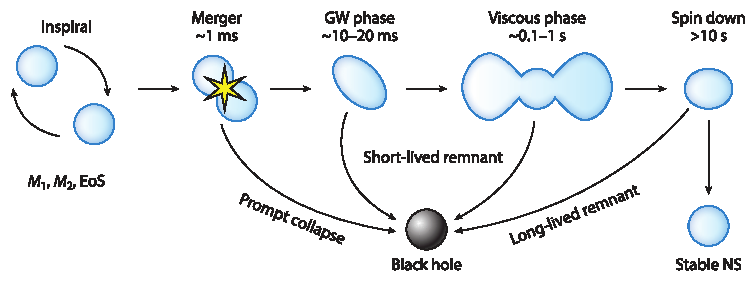
\includegraphics[width=0.60\textwidth]{Fig_3_Rad.pdf}
    \caption{
        Overview of the different phases in an NS merger and the relative timescales. 
        The inspiral ends with the merger, when the two stars start to fuse together. 
        The early \pmerg{} evolution is entirely driven by hydrodynamics and by \ac{GW} emission. 
        If the remnant does not collapse within ${\sim}10-20\,$ms, \ac{GW} losses
        subside and other physical processes become more important: 
        Angular momentum redistribution (which is due to turbulent viscosity) 
        and neutrino losses operate over a timescale of a tenth of a second to a few
        seconds. This is also the characteristic timescale for the evolution of the remnant disk. 
        If the remnant does not collapse over a timescale of a few seconds, then it will 
        spin down because of \ac{MHD} effects over a possibly much longer timescale 
        of several seconds to a few hours. 
        (Adapted from \citet{Radice:2020ddv})
    }
    \label{fig:intro:pic}
\end{figure}

The qualitative picture of the \ac{BNS} merger dynamics is depicted in Fig.~\ref{fig:intro:pic}. 
The main parameters that determine the evolutionary path are the total gravitational mass, 
$M_{\rm tot}$, \mr, $q$, and \ac{EOS}. The intrinsic angular momenta (also called spin) of \acp{NS} 
can be neglected to a certain extend as (i) astrophysical \acp{NS}, observed as pulsars, have 
spin lower than the orbital angular momentum of the system and (ii) the \acp{NS} internal 
viscosity is too low to allow for tidal locking make stars co-rotate \cite{(e.g. Bildsten & Cutler, 1992)}.

It is possible that the object formed after the merger has mass exceeding $M_{\rm max}$. 
The remnant might still avoid the fate of collapsing to a \ac{BH} immediately, if the differential 
rotation is strong enough to provide additional support against gravity. The mass threshold 
for that is rather uncertain but is estimated to be $M_{\rm crit,1}\sim1.3-1.7M_{\rm max}$ 
(e.g. Shibata et al., 2003; Shibata & Taniguchi, 2006). Such an object is commonly referred to as 
\ac{HMNS}. Its lifetime is determined by the rate at which it is loosing energy to, \eg, \acp{GW}
and the angular momentum is being redistributed, making it more compact. 
Another threshhold mass is the maxiumum mass that a rigidly rotating \ac{NS} can have, the 
$M_{\rm crit,2}$ and is $M_{\rm crit,2}{\lesssim}1.2M_{\rm max}$ \cite{Cook et al., 1994}. 
%If the newly formed remnant has mass lower than $M_{\rm crit,2}$, it can in principle survive 
%for 
If the newly formed remnant has mass exceeding $M_{\rm crit,2}$, it is expected to collapse to 
a \ac{BH} after the redistribution of the angular momentum. However, this scenario remains 
unconfirmed as it requires long-term, fully self-consistent investigation with expensive 
\ac{NR} simulations. In this thesis we attempt to constrain this evolutionary path.

After the merger, a remnant, be it a \ac{NS} or a \ac{BH} can be surrounded by a matter, that 
have a different rotation profile, lower density (compare to \ac{NS}) but still gravitationally 
bound to the central object. This matter is generally called disk or torus. Its mass and 
properties are crucial in determining the long-term evolution of the system and \pmerg{} 
outflows. However, they are not well understood on a quantitative level, as long-term 
self-consistent \ac{NR} simulations with advanced physics input that are required for their study 
are very computationally expensive. 
%In this thesis we attempt to advance our understanding of the disk by by means of our 
%own \ac{NR} simulations and via statistical analysis of all the data publicly available from 
%other groups.

%%%% <<< moved from BNS_merg_sims :: ejecta >>> 
When \acp{NS} collide and merger, matter is ejected through a number of 
different physical processes, gaining enough energy to become graviationally 
unbound (according to the criteria discussed in Sec.~\ref{sec:bns_sims:method:ejecta}). 
%\alpedit{The matter ejected on dynamical timescale of the system (${\sim}10$~ms) 
%is called the dynamical ejecta.}{
In particular, the matter ejected within a few dynamical timescales (\ie, ${\sim}10$~ms) 
after merger by tidal torques and hydrodynamics shocks driven by core bounces 
is called \ac{DE} \citep[\eg][]{Hotokezaka:2013b,Bauswein:2013yna,Radice:2016dwd,Radice:2018pdn}. 
%
% From AFTERGLOW paper
%
Several mechanisms contribute to the ejection, and depending on the 
binary parameters, their relative contribution differs.
%
For instance, shortly before and during the merger, the outer parts 
of the \acp{NS}, opposite to the collisional interface, are stripped 
away by the tidal torque and centrifugal forces. This is the tidal 
component of the \ac{DE}. It is more massive in binaries with 
larger \mr{} and is maximum in those that experience tidal disruption 
\citep[\eg][]{Radice:2018pdn,Bernuzzi:2020txg}.
%
Such ejecta is neutron rich, confined largely to the orbital plane and exhibits 
a crescent-like azimuthal structure \citep{Bernuzzi:2020txg}.
%
Overall, the tidal ejecta component is mostly equatorial and its 
velocity is related to the \acp{NS}' velocity at merger and 
and the system's escape velocity, and is $\sim0.2$~c.
%
When \acp{NS}' cores collide and bounce, shocks propagate outwards inducing 
matter ejection. Additionally, a small amount of material at the 
\acp{NS}' collisional interface is shock-heated and launched into the polar 
direction. This comprises the shocked component of the \ac{DE}.
%
It is more massive and faster if \acp{NS}' radii are smaller and they collide 
at higher velocities \citep[\eg][]{Radice:2018pdn}. 
%
Overall the dynamical ejecta has a broad distribution in terms of composition, 
velocity and mass, dependent on the parameters of the binary and \ac{NS} \ac{EOS}.
%% === ON THE FAST DYNAMICAL EJECTA IN PARTICULAR ===========

\red{Might add 'on a longer timescale other ejecta components are expected'}

\subsection{Post-merger remnant}

After the merger, the newly born \ac{MNS} remnant is not axisymmetric. It is 
subjected to dynamical instabilities, that to the large degree define its interaction 
with the surrounding medium and its lifetime. The remnant dies not rotate as a 
single "rigid" body, but instead exhibit the differential rotation, where 
different layers rotate at different angular velocities. This excess in 
angular momentum with respert to the \ac{RNS} provides an additional support 
against gravitational collapse. \acp{GW} can carry away a large amount 
of angular momentum 


\subsection{Accretion disks}

Accretion disks comprise the matter that is orbits the central object near rotational 
equilibrium and accretes onto the central object. Such phenomena can be found in a variety of 
incarnations and on a broad range of spatial scales in the Universe, \eg, around proto-stellar
object during the star formation, in X-ray binaries, when the matter from the massive 
companion star is being accreted onto a compact object, or in \ac{AGN}
\cite{see e.g. Pringle, 1981; Balbus & Hawley, 1998; Spruit, 2010a, for reviews}.
While being studied for a long time via a broad range of methods, the key physical mechanisms, 
that induce the accretion, \ie, the transport of angular momentum, is not well understood.
This problem becomes considerably more complex, when the central object is not axisymmetric 
and interact with the disk. 
One of the mechanisms responsible for the transport of angular momentum, is the torque between
differentially rotating fluid elements exerted by microscopic viscosity. However, it is 
orders of magnitudes weaker than what is required to explain the observed accretion rates 
\cite{e.g. Lust, 1952} 
%Additionally, an effecitve shear streses are generated in the flued
%that is sugjected to stochastic small-scale motions in the flow tih high Reynolds nuimbers.

\paragraph{The $\alpha$-viscosity approximation}

It is possible to describe the disk turbulence without known the exact mechanism responsible 
for it. Shakura \& Sunyaev (1973) \cite{Shakura & Sunyaev (1973)} proposed a method to 
parameterize the shear stress under the assumption that the disk flow is quasi-laminar. 
This is so-called ``turbulent kinematic $\alpha$-viscosity'' model, that can be derived 
from the dimensional analysis. For the characteristic quantities of the local disk medium, 
the sound speed $c_s$ and the Keplerian\footnote{
    By Keplerian we imply a stationary orbit, where the gravitaional attraction is balanced 
    by the centrifugal force exactly.
} angular velocity $\Omega_K$, the $\alpha$-viscocity more reads 
%
\begin{equation}
    \nu_{\rm vis} = \alpha_{\rm vis} \frac{c_{s}^2}{\Omega_K}
\end{equation}
%
where the parameter $\alpha$ controls the ``strength'' of large scale shear stresses that drive 
the accretion. Generally, $\alpha$ is not a constant and depends on local hydrodynamic 
conditions in the disk. While not being a self-consistent, the model is simple and powerful 
and is widely used in studies of accretion disks, \eg, the 
``advection domianted accretion flow'' (ADAF, \cite{Narayan & Yi, 1994}). 
The $\alpha$-model is used to study the geometrically thick accretion disks in 
multi-dimensional time-dependent simulations. It allows to avoid the numerical issues 
related to a more self-consistent, elemental description of the turbulence.
\cite{(e.g. Stone et al., 1999; Igumenshchev et al., 2000 Lee et al., 2005 
Mac-Fadyen & Woosley, 1999; Setiawan et al., 2006}

Origin of the underlying instability behind the disk turbulence, and thus the angular 
momentum transport is not well understood. The purely hydrodynamic instability within 
discs with very large Reynolds numbers reaching ${\sim}10^{14}$ within the flow, was 
not identified, contrary to the ideal shear flows, that are localloy non-linearly unstable 
showing the presence of turbulence \cite{e.g. Orszag & Kells, 1980)}. In disks, the nearly 
Keplerian profile seems to be the stabilizing property \cite{e.g. Balbus & Hawley, 1998)}.
Notably, the discretization of the hydrodynamic equations introduces the so-called 
numerical viscosity (see more detains in Sec.~\ref{sec:nr_methds:visc}) which further 
challenges the interpretation of the numerical models of turbulent flows 
(see \cite{e.g. Lesur & Papaloizou, 2010})


\paragraph{Magnetized accretion disks}

Seed magnetic fields within an accretion disk can be amplified via so-called \ac{MRI} to the 
scales at which they become dynamically important and induce turbulence and magnetic 
shear tension. This, in turn, enhances the angular momentum transport. 
Models of magnetized accretion disks are widely used to study the formation of the 
relativistic jets, that are projenitors of \acp{GRB}. 
Several mechanisms have been proposed. For instance, the 
magneto-centrifugal acceleration mechanism, \cite{e.g. Spruit, 2010b}, where 
the jet is powered by the accretion disk alone, and the Blandford \& Znajek mechanism, 
(BZ-process) where the jet is powered by the rotating central BH, rotational energy from
which is extracted by the Poynting flux of magnetic field directed outward.


\subsection{Post-merger accretion disks}

Having discussed the astrophysical phenomena related to the \pmerg{} evolution of 
the \ac{BNS} systems, we now outline the overall qualitative picture of the physical 
processes operating in this events.

The Remnant is hot and a strong emitter of neutrinos, which are partially absorbed 
and reprocessed by the disk. 
The disk itself is hot, moderately dense with the neutrino rich inner matter, shielded from 
the neutrino irradiation, and proton-rich outer layers. The disk mainly consists of 
electrons, positrons, protons and free nucleons. As the shocks generated at merger 
subside, three main processes starts to dominate the disk evolution: mass and and 
angular momentum exchange with the remnant, expansion and mass-loss at the outer 
boundary, and cooling via neutrino emission. The recombination of the free nucleons 
to helium and heavier nuclei occur at large radii, around few hundred kilometers 
away from the remnant (in comparison with the radius of the remnant that is around 
eleven kilometers). The energy released at this process further facilitates the 
formation of the outflow. While the disk itself is optically and geometrically 
thick, its outer regions are have densities and temperatures low enough so that 
neutrinos can escape, or ``free stream'' once created. This classifies as 
\textit{transparent regime} for the neutrino radiation trapsport. 
Deeper in the disk and closer to the remnant, the densities and temperatures are 
higher and coupling between matter and neutrinos is increased, which leads to 
an increased frequency on neutrino reabsorptions. Thus, neutrinos can transport 
energy and lepton number from the point of creating, in the hot and dense inner 
regions, outwards. The energy deposition can drive subrelativistic wind of 
gravitationally unbound mater, the so-called \nwind{}. \gray{The wind is a place for \rproc{} \nuc{} and EM counterpart} \gray{Additionally, an out
ow could also be powered by means of magnetic-field effects or the energy release from nucleons recombining to $\alpha$-particles.}
At the innermost parts of the disk, the temperatures and densities are so high 
that neutrinos are effectively ``trapped'' by the matter and are advocated by the 
flow. This classifies as \textit{diffusion regime}. The neutrinos ability to 
cool the disk is determined mostly by time it takes for neutrinos to diffuse out,
the so-called \textit{diffusion timescale}.

In addition to participating in the energy transport within the disk, neutrinos 
introduce large amount of energy to the polar region, above the remnant via 
neutrino-anti-neutrino annihilation. This process results in the creation of 
electron-position fireball, that can be energetic enough to initiate \ac{SGRB}. 
The main requirement for that to happen is the low baryon polution of the polar 
region to allow the sufficient deposition of the eneergy per baryong to create the 
untrarelativisitc outflow. In that regard, BH-disk systems appear to be more 
straightforward candidate for the \ac{SGRB} projenitors, as a newly formed \ac{BH} 
provides a natural sink to the material in the polar region. 
Additionally, magnetic fields could play an important role in ``cleaning-up'' the 
polar region and forming a collimated outflow by means of BZ-process. 
Notably, the jet formation is one of the key, not well understood processes 
related to \ac{BNS} mergers.


\section{Previous works}

\acp{BNS} mergers have been studied as a possible cite of \rproc{} \nuc{} 
since `70s \citep{Lattimer:1974a,Symbalisty:1982a,Rosswog:1998hy,Freiburghaus:1999,Rosswog:2005su}. 

The radioactive decay of $r$-process elements produces a
characteristic electromagnetic (EM) transient in the UV/optical/NIR
bands, called kilonova (kN) \citep{Li:1998bw,Kulkarni:2005jw,Metzger:2010sy,Roberts:2011xz,Kasen:2013xka},
that was observed as counterpart of the gravitational-wave event GW170817 \citep{Abbott:2017wuw,Abbott:2017oio,Abbott:2018wiz,Abbott:2018hgk}
and it was named AT2017gfo
\citep{Arcavi:2017xiz,Coulter:2017wya,Drout:2017ijr,Evans:2017mmy,Hallinan:2017woc,Kasliwal:2017ngb,Nicholl:2017ahq,Smartt:2017fuw,Soares-santos:2017lru,Tanvir:2017pws,Troja:2017nqp,Mooley:2018dlz,Ruan:2017bha,Lyman:2018qjg}.
The NIR luminosity of AT2017gfo peaked at several days after the
merger \citep{Chornock:2017sdf}, and it is consistent with the expectation
that the opacities of expanding $r$-process material are dominated by 
lanthanides and possibly actinides \citep{Kasen:2013xka}.  
The UV/optical luminosity peaked instead less than one day after the
merger \citep{Nicholl:2017ahq}, and it originates from ejected material
that experienced only a partial $r$-process nucleosynthesis
\citep{Martin:2015hxa}.

The ejecta masses inferred from observations \citep{Cowperthwaite:2017dyu,Villar:2017wcc,Tanvir:2017pws,Tanaka:2017qxj,Perego:2017wtu,Kawaguchi:2018ptg} are not compatible with those predicted by numerical simulations with targeted neutron star (NS) masses, and several questions remain open. 
In particular, understanding the early blue kN remains a challenging
aspect to explain for most models.
Both semi-analytical and radiation transport
models require large ejecta velocities and electron fractions ($Y_e$'s),
different from those found in simulations,
\citep[\eg][]{Fahlman:2018llv,Nedora:2019jhl}.
The late red kN component requires ejecta masses generally
not observed for the dynamical ejecta computed in numerical relativity (NR) simulations \citep{Radice:2018pdn}. 
In addition, the number of components and the geometry of the emission can have a significant 
effect on the ejecta parameters 
\citep{Perego:2017wtu,Kawaguchi:2018ptg}. Also, it is important to note that the photon diffusion and
emission is often simplified in semi-analytical kN models \citep[\eg][]{Villar:2017wcc,Perego:2017wtu,Siegel:2019mlp}, and  
more accurate radiation transfer computations may alter the inferred ejecta parameters 
\citep{Kawaguchi:2018ptg,Korobkin:2020spe}. However, photon radiation transfer simulations often employ ad-hoc, simplified ejecta different from those computed from ab-initio simulations. 

%% NR methods & dynamical ejecta
Key for interpreting BNS electromagnetic emissions is the detailed modeling of
the mass ejection from BNS mergers, which must include general
relativity, a microphysical equation of states (EOS) of strongly interacting
matter, relativistic (magneto-)hydrodynamics, and neutrino
transport. NR simulations performed so far
mostly focused on the dynamical ejecta that are launched during merger
by tidal torques (tidal component) and by the shocks generated by the
bounce of the NS cores (shocked component),
\citep[\eg][]{Hotokezaka:2013iia,Bauswein:2013yna,Wanajo:2014wha,Sekiguchi:2015dma,Radice:2016dwd,Sekiguchi:2016bjd,Radice:2018pdn,Vincent:2019kor}. In
equal-mass mergers, the shocked component is found to be a factor
${\sim}10$ more massive than the tidal component. This is in
contrast to early works that employed Newtonian gravity and in which
the tidal component dominated the ejecta due to the weaker gravity and
stiffer EOS employed in those simulations
\citep{Ruffert:1996by,Rosswog:1998hy,Rosswog:2001fh,Rosswog:2003rv,Rosswog:2003tn,Rosswog:2003ts,Oechslin:2006uk,Rosswog:2013kqa,Korobkin:2012uy}.
However, even the dynamical ejecta found in NR simulations cannot account alone for the
bright blue and late red components of the observed kN in AT2017gfo \citep{Siegel:2019mlp}.

Winds originating from the merger remnant on timescales of
$\O(0.1-1\,{\rm s})$ can unbind $O(0.1\, \Msun)$ from the remnant and
represent (if present) the largest contribution to the kilonova signal
\citep{Dessart:2008zd,Fernandez:2014bra,Just:2014fka,Lippuner:2017bfm,Siegel:2017nub,Fujibayashi:2017puw,Radice:2018xqa,Fernandez:2018kax,Janiuk:2019rrt,Miller:2019dpt,Fujibayashi:2020qda,Mosta:2020hlh}.
Thus far, these winds have been mostly studied by means of long-term
Newtonian simulations of neutrino-cooled disks, assuming simplified
initial conditions, \citep[\eg]{Metzger:2008av,Beloborodov:2008nx,Lee:2009uc,Fernandez:2012kh}.
Ab-initio (3+1)D NR simulations of the merger with weak-interactions and
magnetohydrodynamics are not yet fully developed at sufficiently long timescales \citep{Sekiguchi:2011zd,Wanajo:2014wha,Sekiguchi:2015dma,Palenzuela:2015dqa,Radice:2016dwd,Lehner:2016lxy,Sekiguchi:2016bjd,Foucart:2016vxd,Bovard:2017mvn,Fujibayashi:2017puw,Fujibayashi:2017xsz,Radice:2018xqa,Nedora:2019jhl,Vincent:2019kor,Bernuzzi:2020txg}.
These simulations are essential to interpret AT2017gfo and future events.
For example, long-term (up to $100$~ms postmerger) NR simulations 
pointed out the existence of \swind{} in which there are
favourable conditions (large ejecta mass, high-velocity and not extremely neutron rich conditions) 
for the early emission from lanthanide poor material \citep{Nedora:2019jhl}.
Such mass ejection can also be boosted by global large-scale magnetic
stresses \citep{Metzger:2018uni,Siegel:2017jug,Siegel:2017nub},
although significant mass fluxes can only be achieved by fine-tuning
initial configuration or setting unrealistic strength of the magnetic
field \citep[\eg][]{Ciolfi:2020hgg,Mosta:2020hlh}.
A third contribution can come from neutrino-driven winds of mass ${\sim} 10^{-4}-10^{-3}M_{\odot}$ originating above the remnant, 
but their mass cannot account for bright signals \citep{Dessart:2008zd,Perego:2014fma,Just:2014fka}.

The nucleosynthesis from BNS mergers is believed to provide a major
contribution to the $r$-process material in the Universe.
However, whether or not BNS mergers are the only source is still debated and 
possible additional $r$-process sites, such as collapsars, 
jet-driven supernovae, and neutron star implosions, have been proposed
\citep{Argast:2003he,Duan:2010af,Winteler:2012hu,Nishimura:2015nca,Hirai:2015npa,Bramante:2016mzo,Nishimura:2016hak,Fuller:2017uyd,Mosta:2017geb,Siegel:2018zxq,Ji:2019ssk,Bartos:2019twj,vandeVoort:2019bxg,Wehmeyer:2019ovu,Vassh:2019cey}.
In particular, it is not clear if BNS mergers can explain r-process enriched ultra-faint dwarf galaxies,
classical dwarf galaxies \citep{Ji:2015wzg,Bramante:2016mzo,Safarzadeh:2018ent,Safarzadeh:2018fdy,Skuladottir:2019bjz,Bonetti:2019fxj}, 
and the evolution of $r$-process abundances both at early and late times \citep{Safarzadeh:2017riw,Safarzadeh:2018ent,Bonetti:2018nwo,Cote:2018qku,Hotokezaka:2018aui,Banerjee:2020eak}


%\red{biased for Shibata papers [from his 2019 paper with hotokezaka]}
%
%Mergers if neutron star binaries (binary neutron stars (BNS)) and neutron star-black hole 
%(NSBH) are one of the most promising sources of graviational waves (GWs) for ground-based
%detectors (\eg, Advanced LIGO and Virgo, and KAGRA \citep{Abadie:2010hv,Accadia:2010aa,Akutsu:2017kpk}).
%On August 17, 2017 advanced LIGO and Aadvanced Virgo made the first observation of GWs from a binary 
%neutron star merger, the event \GW{}. It is expected that advanced GW observatories will detect more
%events such as \GW{} in the near future.
%
%It is expected that a significant amount of matter is ejected during the neutron star merger. 
%This neutron-rich matter, the ejecta, is a promising site for the rapid neutron racture 
%nucleosynthesis, ($r$-process, see sec.\ref{sef:nucleo}), responsible for the creation of the 
%heaviest elements in the Universe \citep{Lattimer:1974slx,Eichler:1989ve,Thielemann:2017acv}.
%Related to the neutron-rich heavy element synthesis in the ejecta, an electromagnetic (EM) transient
%(Kilonova/mactronova) is expected to be powered by the radioactive decay of the \rproc{} 
%elements \citep{Li:1998bw,Metzger:2010,Roberts:2011,Goriely:2011vg,Korobkin:2012uy,Barnes:2013wka,Tanaka:2013ana}.
%This is the electromagnetic counterpart to the gravitational waves from BNS that, if detected, 
%could constrain aid with the source sky localization and allow further constrain models 
%of the chemical evolution and origin of the heavy \rproc{} elements 
%This is supported by the recent observation of ultra-violet, optical, and infrared signals of
%\GW{} \citep{TheLIGOScientific:2017qsa,Tanaka:2017qxj,Arcavi:2017xiz,Coulter:2017wya,Cowperthwaite:2017dyu,Drout:2017ijr,Evans:2017mmy,Kasliwal:2018fwk,Pian:2017gtc,Smartt:2017fuw,Tanvir:2017pws}. 
%In addition to the nuclear decay powered EM counterpart, a long-lasting synchrotron emission 
%is multi-wavelengths is expected from the merger ejecta propagating through the interstellar
%medium (ISM) \citep{Nakar:2011cw}. 
%Such signal, if detected, would provide an additional information on the merger ejecta velocity profile,
%unafeccted by the ill-constrained details of the \rproc{} nucleosynthesis. 
%
%In order to perform a quantitative studies of the aforementioned topics, first the main aspects 
%of the BNS merger have to clarified. These aspects include the merger process, the mass ejection, 
%the nucleosynthesis and subsequent decay of the heavy elements in the ejecta, and EM emission
%arising from the ejecta. Numerical relativity simulations that include accurate microphysical processes, 
%neutrino radiation transport and magnetohydrodynamics (MHD) are the best tool in this regard. 
%
%Owing to the recent rapid advancement in the field of modeling the BNS in numerical-relativity (NR) 
%the detailed simulations of the mergers are now achievable.
%This allowed to investigate the effects of the neutron star matter equation of state, (EOS) that 
%take into account the finite-temperature effects \citep{Duez:2009yz,Sekiguchi:2011zd},
%the effects of the neutrino cooling \citep{Sekiguchi:2011zd,Deaton:2013sla,Foucart:2014nda,Palenzuela:2015dqa} and neutrino heating \citep{Sekiguchi:2015dma,Foucart:2016rxm}, and
%MHD instability \citep{Kiuchi:2014hja,Kiuchi:2015sga,Kiuchi:2015sga}.
%Numerical relativity simulations are currently the best way to study the mergers and predict the features, 
%that can be tested with later observations.
%
%In BNS mergers the mass ejection processes have been studied with NR simulations have been first 
%investigated by \citet{Hotokezaka:2013b} while in the NSBH mergers by \citet{Foucart:2012vn}. A large number of numerical relativity 
%simulations have been performed to study the nature of the first material that is being ejected 
%on the dynamical timescale (the dynamical ejecta) \citep{Sekiguchi:2015dma,Palenzuela:2015dqa,Lovelace:2013vma,Kyutoku:2013wxa,Foucart:2015vpa,Foucart:2015gaa,Foucart:2016rxm,Sekiguchi:2016bjd,Lehner:2016lxy,Radice:2016dwd,Foucart:2016vxd,Kyutoku:2017voj,Dietrich:2018uni,Dietrich:2016lyp,Bovard:2017mvn,Radice:2018pdn}. This works showed that ejecta mass depends on the binary parameters, such as mass ration, and on 
%the EOS. The ejecta was found to host material with broad range of compositions, where the latter 
%is usually quantified with electron fraction $Y_e$, which is the electron number density per baryon 
%number density. This wide range of $Y_e$, is however consistent with the observed abundance patterns 
%of \rproc{} elements (with mass number larger $A\sim90$) in the Solar System and metal poor-stars \citep{Wanajo:2014wha,Radice:2016dwd}.
%
%After a BNS merger, a remnant is born. It can be a black hole (BH) or a massive, stable or unstable, neutron star (MNS). Both could be surrounded by a gravitationally bound matter, a disk (torus). 
%The \pmerg{} evolution have been investigated by many groups \citep{Fernandez:2013tya,Metzger:2014ila,Perego:2014fma,Fernandez:2014cna,Just:2014fka,Fernandez:2016sbf,Siegel:2017nub,Fujibayashi:2017xsz,Fernandez:2018kax}. 
%Simulations showed that a certain fraction of the disk can become unbound, and be ejected from the system, 
%by viscous, nuclear recombination or MHD effects. 
%This long-term ejecta was found to be more massive then the dynamical ejecta in certain cases and thus,
%even more important for EM counterparts and nucleosynthetic yields.
%
%In this thesis we discuss the numerical relativity simulations performed with the code \texttt{WhiskyTHC}
%
%
%
%In this thesis we perform and analyze numerical relativity simulations of merging neutron stars. 
%These simulations are performed via solving the equations of general relativity, hydrodynamics and radiation, neutrino, transport via special numerical schemes. 
%
%In this chapter we provide a brief description of the main equations and methods used to produce simulations analyzed in this thesis. 
%For the sace of bravity we limit the discussion to the main results and implication important for our work.
%For the underlying principles of the Eintein's theory of General Relativity, for which we here the reado to \red{[GR refs]}.
%For the discussion and derivation of general relativistic hydrodynamics and refer the interested reader to \red{[GRHD refs]}.
%For the Discussion on the radiation transport we refer to \red{GR-Rad refs}
%
%%% from GRLES Raduce paper
%Multimessenger observations of BNS mergers are starting to constrain the poorly known properties of
%matter at extreme densities [11,12,20–36] and the physical processes powering short g-ray bursts (SGRBs)
%[37–42]. They are also beginning to reveal the role played by compact binary mergers in the chemical
%enrichment of the galaxy with r-process elements [8,13,43–62]. The key to the solution of some of the most
%pressing open problems in nuclear and high-energy astrophysics – such as the origin of heavy elements,
%the nature of neutron stars (NSs), and the origin of SGRBs – is encoded in these and future observations.
%However, theory is essential to turn observations into answers.

\section{Aims and organization of this thesis}

A \pmerg{} \ac{MNS}-disk system hosts a variety of interesting physics, most of which are 
are currently not well understood.
